This section describes the data files for a \mf Groundwater Transport (GWT) Model.  A GWT Model is added to the simulation by including a GWT entry in the MODELS block of the simulation name file.

There are three types of spatial discretization approaches that can be used with the GWT Model: DIS, DISV, and DISU.  The input instructions for these three packages are not described here in this section on GWT Model input; input instructions for these three packages are described in the section on GWF Model input.

The GWT Model is designed to permit input to be gathered, as it is needed, from many different files.  Likewise, results from the model calculations can be written to a number of output files. The GWT Model Listing File is a key file to which the GWT model output is written.  As \mf runs, information about the GWT Model is written to the GWT Model Listing File, including much of the input data (as a record of the simulation) and calculated results.  Details about the files used by each package are provided in this section on the GWT Model Instructions.

The GWT Model reads a file called the Name File, which specifies most of the files that will be used in a simulation. Several files are always required whereas other files are optional depending on the simulation. The Output Control Package receives instructions from the user to control the amount and frequency of output.  Details about the Name File and the Output Control Package are described in this section.

\subsection{Multi-Species Transport Simulation}
The present implementation of the GWT Model does not directly support transport of multiple solute species.  However, a simulation can include multiple models, including multiple GWT models.  Thus, multi-species transport simulations are possible by using a separate GWT model for each species.

\subsection{Units of Length and Time}
The GWF Model formulates the groundwater flow equation without using prescribed length and time units. Any consistent units of length and time can be used when specifying the input data for a simulation. This capability gives a certain amount of freedom to the user, but care must be exercised to avoid mixing units.  The program cannot detect the use of inconsistent units.

\subsection{Steady-State Simulations}
A steady-state transport simulation is represented by a single stress period having a single time step with the storage term set to zero. Setting the number and length of stress periods and time steps is the responsibility of the Timing Module of the \mf framework.

TODO: Need to implement mixed steady state and transient periods

\subsection{Solute Mass Budget}
A summary of all inflow (sources) and outflow (sinks) of solute mass is called a mass budget.  \mf calculates a mass budget for the overall model as a check on the acceptability of the solution, and to provide a summary of the sources and sinks of mass to the flow system.  The solute mass budget is printed to the GWT Model Listing File for selected time steps.

\subsection{Time Stepping}


\newpage
\subsection{GWT Model Name File}
The GWT Model Name File specifies the options and packages that are active for a GWT model.  The Name File contains two blocks: OPTIONS  and PACKAGES. The length of each line must be 299 characters or less. The lines in each block can be in any order.  Files listed in the PACKAGES block must exist when the program starts. 

Comment lines are indicated when the first character in a line is one of the valid comment characters.  Commented lines can be located anywhere in the file. Any text characters can follow the comment character. Comment lines have no effect on the simulation; their purpose is to allow users to provide documentation about a particular simulation. 

\vspace{5mm}
\subsubsection{Structure of Blocks}
\lstinputlisting[style=blockdefinition]{./mf6ivar/tex/gwt-nam-options.dat}
\lstinputlisting[style=blockdefinition]{./mf6ivar/tex/gwt-nam-packages.dat}

\vspace{5mm}
\subsubsection{Explanation of Variables}
\begin{description}
% DO NOT MODIFY THIS FILE DIRECTLY.  IT IS CREATED BY mf6ivar.py 

\item \textbf{Block: OPTIONS}

\begin{description}
\item \texttt{list}---is name of the listing file to create for this GWT model.  If not specified, then the name of the list file will be the basename of the GWT model name file and the '.lst' extension.  For example, if the GWT name file is called ``my.model.nam'' then the list file will be called ``my.model.lst''.

\item \texttt{PRINT\_INPUT}---keyword to indicate that the list of all model stress package information will be written to the listing file immediately after it is read.

\item \texttt{PRINT\_FLOWS}---keyword to indicate that the list of all model package flow rates will be printed to the listing file for every stress period time step in which ``BUDGET PRINT'' is specified in Output Control.  If there is no Output Control option and ``PRINT\_FLOWS'' is specified, then flow rates are printed for the last time step of each stress period.

\item \texttt{SAVE\_FLOWS}---keyword to indicate that all model package flow terms will be written to the file specified with ``BUDGET FILEOUT'' in Output Control.

\end{description}
\item \textbf{Block: PACKAGES}

\begin{description}
\item \texttt{ftype}---is the file type, which must be one of the following character values shown in table~\ref{table:ftype}. Ftype may be entered in any combination of uppercase and lowercase.

\item \texttt{fname}---is the name of the file containing the package input.  The path to the file should be included if the file is not located in the folder where the program was run.

\item \texttt{pname}---is the user-defined name for the package. PNAME is restricted to 16 characters.  No spaces are allowed in PNAME.  PNAME character values are read and stored by the program for stress packages only.  These names may be useful for labeling purposes when multiple stress packages of the same type are located within a single GWT Model.  If PNAME is specified for a stress package, then PNAME will be used in the flow budget table in the listing file; it will also be used for the text entry in the cell-by-cell budget file.  PNAME is case insensitive and is stored in all upper case letters.

\end{description}


\end{description}

\begin{table}[H]
\caption{Ftype values described in this report.  The \texttt{Pname} column indicates whether or not a package name can be provided in the name file.  The capability to provide a package name also indicates that the GWT Model can have more than one package of that Ftype}
\small
\begin{center}
\begin{tabular*}{\columnwidth}{l l l}
\hline
\hline
Ftype & Input File Description & \texttt{Pname}\\
\hline
DIS6 & Rectilinear Discretization Input File \\
DISV6 & Discretization by Vertices Input File \\
DISU6 & Unstructured Discretization Input File \\
FMI6 & Flow Model Interface Package &  \\ 
IC6 & Initial Conditions Package \\
OC6 & Output Control Option \\
ADV6 & Advection Package \\ 
DSP6 & Dispersion Package \\ 
SSM6 & Source and Sink Mixing Package \\ 
MST6 & Mobile Storage and Transfer Package \\
IST6 & Immobile Storage and Transfer Package & * \\
CNC6 & Constant Concentration Package & * \\ 
SRC6 & Mass Source Loading Package & * \\ 
LKT6 & Lake Transport Package & * \\ 
SFT6 & Streamflow Transport Package & * \\ 
MWT6 & Multi-Aquifer Well Transport Package & * \\ 
UZT6 & Unsaturated Zone Transport Package & * \\ 
MVT6 & Mover Transport Package \\ 
OBS6 & Observations Option \\
\hline 
\end{tabular*}
\label{table:ftype}
\end{center}
\normalsize
\end{table}

\vspace{5mm}
\subsubsection{Example Input File}
\lstinputlisting[style=inputfile]{./mf6ivar/examples/gwt-nam-example.dat}



%\newpage
%\subsection{Structured Discretization (DIS) Input File}
%Discretization information for structured grids is read from the file that is specified by ``DIS6'' as the file type.  Only one discretization input file (DISU6, DISV6 or DIS6) can be specified for a model.

\vspace{5mm}
\subsubsection{Structure of Blocks}
\lstinputlisting[style=blockdefinition]{./mf6ivar/tex/gwf-dis-options.dat}
\lstinputlisting[style=blockdefinition]{./mf6ivar/tex/gwf-dis-dimensions.dat}
\lstinputlisting[style=blockdefinition]{./mf6ivar/tex/gwf-dis-griddata.dat}

\vspace{5mm}
\subsubsection{Explanation of Variables}
\begin{description}
% DO NOT MODIFY THIS FILE DIRECTLY.  IT IS CREATED BY mf6ivar.py 

\item \textbf{Block: OPTIONS}

\begin{description}
\item \texttt{length\_units}---is the length units used for this model.  Values can be ``FEET'', ``METERS'', or ``CENTIMETERS''.  If not specified, the default is ``UNKNOWN''.

\item \texttt{NOGRB}---keyword to deactivate writing of the binary grid file.

\item \texttt{xorigin}---x-position of the lower-left corner of the model grid.  A default value of zero is assigned if not specified.  The value for XORIGIN does not affect the model simulation, but it is written to the binary grid file so that postprocessors can locate the grid in space.

\item \texttt{yorigin}---y-position of the lower-left corner of the model grid.  If not specified, then a default value equal to zero is used.  The value for YORIGIN does not affect the model simulation, but it is written to the binary grid file so that postprocessors can locate the grid in space.

\item \texttt{angrot}---counter-clockwise rotation angle (in degrees) of the lower-left corner of the model grid.  If not specified, then a default value of 0.0 is assigned.  The value for ANGROT does not affect the model simulation, but it is written to the binary grid file so that postprocessors can locate the grid in space.

\end{description}
\item \textbf{Block: DIMENSIONS}

\begin{description}
\item \texttt{nlay}---is the number of layers in the model grid.

\item \texttt{nrow}---is the number of rows in the model grid.

\item \texttt{ncol}---is the number of columns in the model grid.

\end{description}
\item \textbf{Block: GRIDDATA}

\begin{description}
\item \texttt{delr}---is the is the column spacing in the row direction.

\item \texttt{delc}---is the is the row spacing in the column direction.

\item \texttt{top}---is the top elevation for each cell in the top model layer.

\item \texttt{botm}---is the bottom elevation for each cell.

\item \texttt{idomain}---is an optional array that characterizes the existence status of a cell.  If the IDOMAIN array is not specified, then all model cells exist within the solution.  If the IDOMAIN value for a cell is 0, the cell does not exist in the simulation.  Input and output values will be read and written for the cell, but internal to the program, the cell is excluded from the solution.  If the IDOMAIN value for a cell is 1, the cell exists in the simulation.  If the IDOMAIN value for a cell is -1, the cell does not exist in the simulation.  Furthermore, the first existing cell above will be connected to the first existing cell below.  This type of cell is referred to as a ``vertical pass through'' cell.

\end{description}


\end{description}

\vspace{5mm}
\subsubsection{Example Input File}
\lstinputlisting[style=inputfile]{./mf6ivar/examples/gwf-dis-example.dat}


%\newpage
%\subsection{Discretization with Vertices (DISV) Input File}
%Discretization information for DISV grids is read from the file that is specified by ``DISV6'' as the file type.  Only one discretization input file (DISV6, DISU6 or DIS6) can be specified for a model.

The approach for numbering cell and cell vertices for the DISV Package is shown in figure~\ref{fig:gwf-fig3-2}.  The list of vertices for a cell must be in clockwise order.  Closing of the cell polygon by repeating the first vertex as the last vertex is not required in the present implementation.  Internally within the program, however, the first vertex number is added to the end of the vertex list in order to close the polygon.  Thus, users have the option for whether or not to close cell polygons.

\begin{figure}[ht]
	\centering
	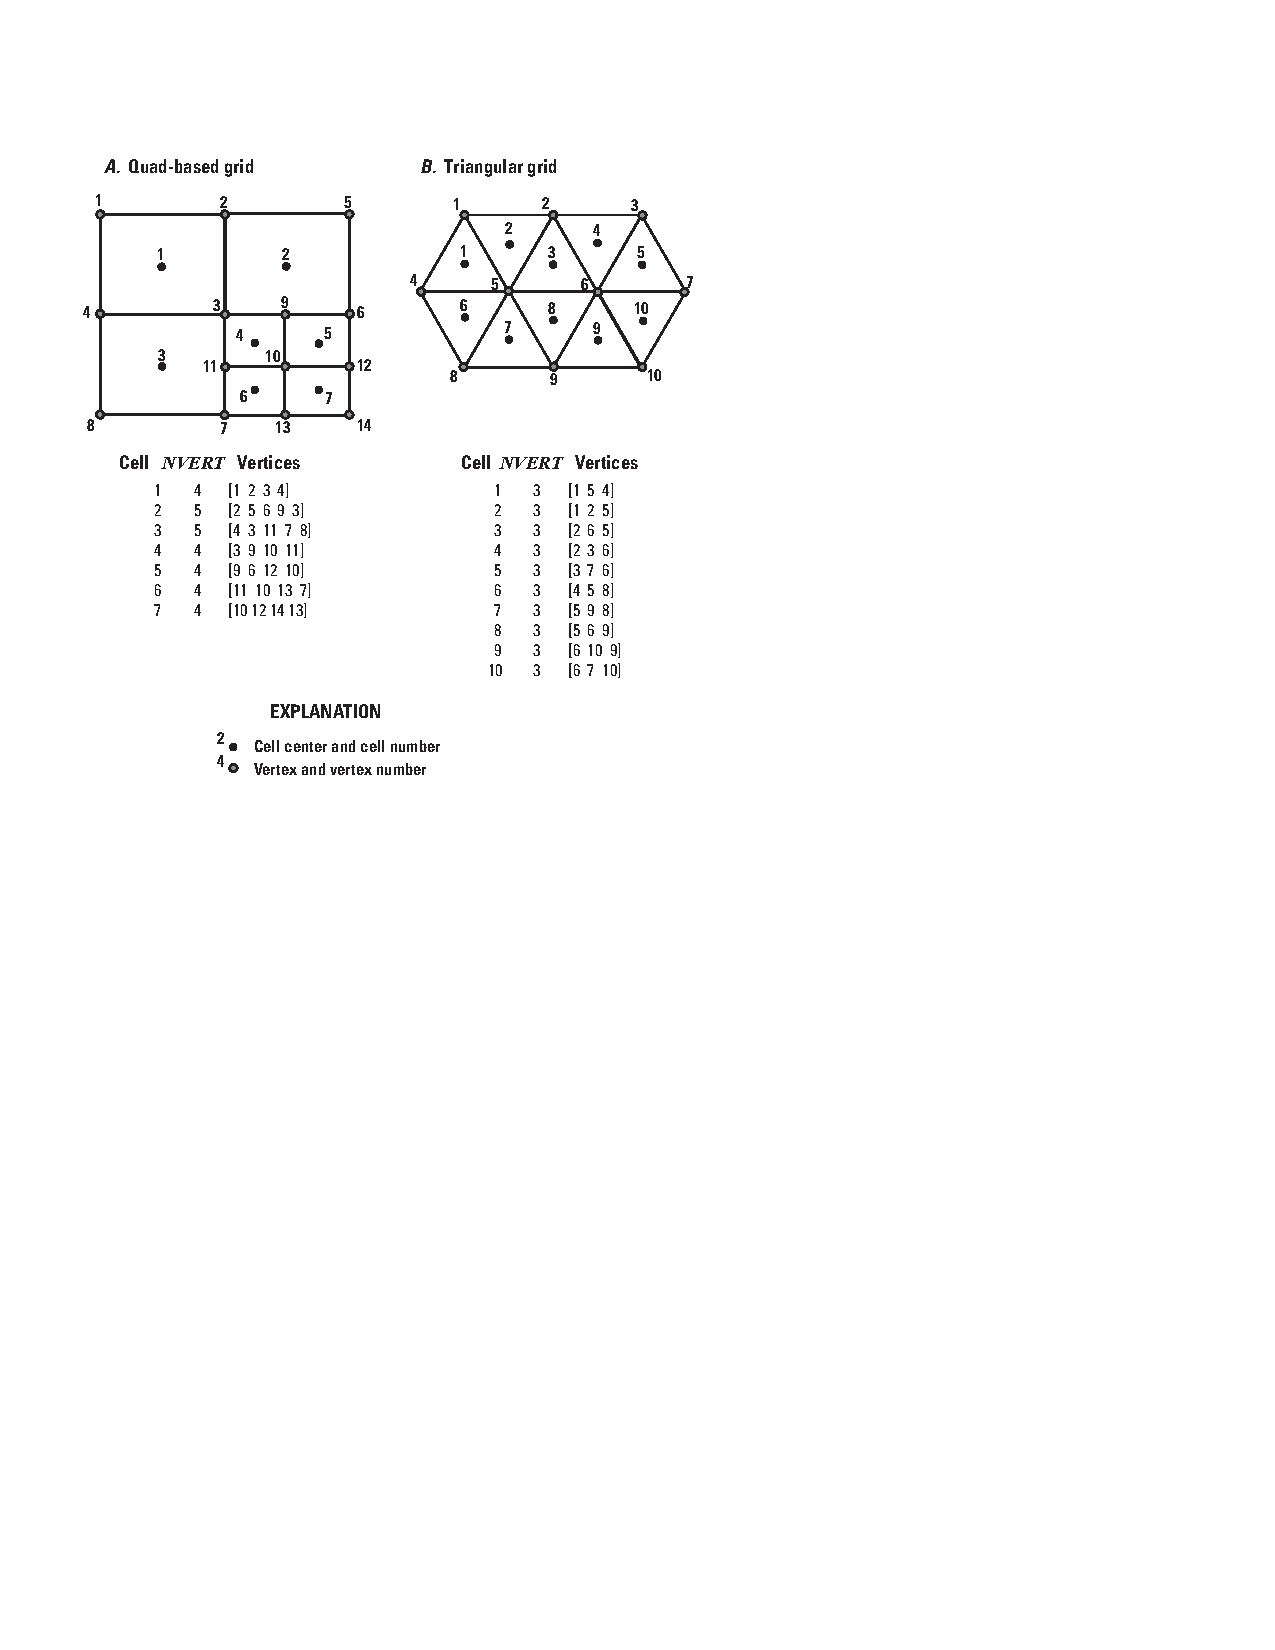
\includegraphics[scale=1.0]{gwf-fig3-2}
	\caption{Schematic diagram showing the vertices and cells defined using the Discretization by Vertices Package. The list of vertices used to define each cell must be in clockwise order.  From \cite{modflow6gwf}}
	\label{fig:gwf-fig3-2}
\end{figure}


\vspace{5mm}
\subsubsection{Structure of Blocks}
\lstinputlisting[style=blockdefinition]{./mf6ivar/tex/gwf-disv-options.dat}
\lstinputlisting[style=blockdefinition]{./mf6ivar/tex/gwf-disv-dimensions.dat}
\lstinputlisting[style=blockdefinition]{./mf6ivar/tex/gwf-disv-griddata.dat}
\lstinputlisting[style=blockdefinition]{./mf6ivar/tex/gwf-disv-vertices.dat}
\lstinputlisting[style=blockdefinition]{./mf6ivar/tex/gwf-disv-cell2d.dat}

\vspace{5mm}
\subsubsection{Explanation of Variables}
\begin{description}
% DO NOT MODIFY THIS FILE DIRECTLY.  IT IS CREATED BY mf6ivar.py 

\item \textbf{Block: OPTIONS}

\begin{description}
\item \texttt{length\_units}---is the length units used for this model.  Values can be ``FEET'', ``METERS'', or ``CENTIMETERS''.  If not specified, the default is ``UNKNOWN''.

\item \texttt{NOGRB}---keyword to deactivate writing of the binary grid file.

\item \texttt{xorigin}---x-position of the origin used for model grid vertices.  This value should be provided in a real-world coordinate system.  A default value of zero is assigned if not specified.  The value for \texttt{xorigin} does not affect the model simulation, but it is written to the binary grid file so that postprocessors can locate the grid in space.

\item \texttt{yorigin}---y-position of the origin used for model grid vertices.  This value should be provided in a real-world coordinate system.  If not specified, then a default value equal to zero is used.  The value for \texttt{yorigin} does not affect the model simulation, but it is written to the binary grid file so that postprocessors can locate the grid in space.

\item \texttt{angrot}---counter-clockwise rotation angle (in degrees) of the model grid coordinate system relative to a real-world coordinate system.  If not specified, then a default value of 0.0 is assigned.  The value for \texttt{angrot} does not affect the model simulation, but it is written to the binary grid file so that postprocessors can locate the grid in space.

\end{description}
\item \textbf{Block: DIMENSIONS}

\begin{description}
\item \texttt{nlay}---is the number of layers in the model grid.

\item \texttt{ncpl}---is the number of cells per layer.  This is a constant value for the grid and it applies to all layers.

\item \texttt{nvert}---is the total number of (x, y) vertex pairs used to characterize the horizontal configuration of the model grid.

\end{description}
\item \textbf{Block: GRIDDATA}

\begin{description}
\item \texttt{top}---is the top elevation for each cell in the top model layer.

\item \texttt{botm}---is the bottom elevation for each cell.

\item \texttt{idomain}---is an optional array that characterizes the existence status of a cell.  If the \texttt{idomain} array is not specified, then all model cells exist within the solution.  If the \texttt{idomain} value for a cell is 0, the cell does not exist in the simulation.  Input and output values will be read and written for the cell, but internal to the program, the cell is excluded from the solution.  If the \texttt{idomain} value for a cell is 1, the cell exists in the simulation.  If the \texttt{idomain} value for a cell is -1, the cell does not exist in the simulation.  Furthermore, the first existing cell above will be connected to the first existing cell below.  This type of cell is referred to as a ``vertical pass through'' cell.

\end{description}
\item \textbf{Block: VERTICES}

\begin{description}
\item \texttt{iv}---is the vertex number.  Records in the VERTICES block must be listed in consecutive order from 1 to \texttt{nvert}.

\item \texttt{xv}---is the x-coordinate for the vertex.

\item \texttt{yv}---is the y-coordinate for the vertex.

\end{description}
\item \textbf{Block: CELL2D}

\begin{description}
\item \texttt{icell2d}---is the cell2d number.  Records in the CELL2D block must be listed in consecutive order from 1 to \texttt{ncpl}.

\item \texttt{xc}---is the x-coordinate for the cell center.

\item \texttt{yc}---is the y-coordinate for the cell center.

\item \texttt{ncvert}---is the number of vertices required to define the cell.  There may be a different number of vertices for each cell.

\item \texttt{icvert}---is an array of integer values containing vertex numbers (in the VERTICES block) used to define the cell.  Vertices must be listed in clockwise order.  Cells that are connected must share vertices.

\end{description}


\end{description}

\vspace{5mm}
\subsubsection{Example Input File}
\lstinputlisting[style=inputfile]{./mf6ivar/examples/gwf-disv-example.dat}


%\newpage
%\subsection{Unstructured Discretization (DISU) Input File}
%Discretization information for unstructured grids is read from the file that is specified by ``DISU6'' as the file type.  Only one discretization input file (DISU6, DISV6 or DIS6) can be specified for a model.

The shape and position of each cell can be defined using vertices.  This information is optional and is only read if the number of vertices (NVERT) in the DIMENSIONS block is specified and is assigned a value larger than zero.  If the vertices and two-dimensional cell information is provided in this file, then this information is also written to the binary grid file.  Providing this information may be useful for other postprocessing programs that read the binary grid file.

The DISU Package does not support the concept of layers, which is different from the DISU implementation in MODFLOW-USG.  In \mf~all grid input and output for models that use the DISU Package is entered or written as a one-dimensional array of size nodes.

\vspace{5mm}
\subsubsection{Structure of Blocks}
\lstinputlisting[style=blockdefinition]{./mf6ivar/tex/gwf-disu-options.dat}
\lstinputlisting[style=blockdefinition]{./mf6ivar/tex/gwf-disu-dimensions.dat}
\lstinputlisting[style=blockdefinition]{./mf6ivar/tex/gwf-disu-griddata.dat}
\lstinputlisting[style=blockdefinition]{./mf6ivar/tex/gwf-disu-connectiondata.dat}
\lstinputlisting[style=blockdefinition]{./mf6ivar/tex/gwf-disu-vertices.dat}
\lstinputlisting[style=blockdefinition]{./mf6ivar/tex/gwf-disu-cell2d.dat}

\vspace{5mm}
\subsubsection{Explanation of Variables}
\begin{description}
% DO NOT MODIFY THIS FILE DIRECTLY.  IT IS CREATED BY mf6ivar.py 

\item \textbf{Block: OPTIONS}

\begin{description}
\item \texttt{length\_units}---is the length units used for this model.  Values can be ``FEET'', ``METERS'', or ``CENTIMETERS''.  If not specified, the default is ``UNKNOWN''.

\item \texttt{NOGRB}---keyword to deactivate writing of the binary grid file.

\item \texttt{xorigin}---x-position of the origin used for model grid vertices.  This value should be provided in a real-world coordinate system.  A default value of zero is assigned if not specified.  The value for XORIGIN does not affect the model simulation, but it is written to the binary grid file so that postprocessors can locate the grid in space.

\item \texttt{yorigin}---y-position of the origin used for model grid vertices.  This value should be provided in a real-world coordinate system.  If not specified, then a default value equal to zero is used.  The value for YORIGIN does not affect the model simulation, but it is written to the binary grid file so that postprocessors can locate the grid in space.

\item \texttt{angrot}---counter-clockwise rotation angle (in degrees) of the model grid coordinate system relative to a real-world coordinate system.  If not specified, then a default value of 0.0 is assigned.  The value for ANGROT does not affect the model simulation, but it is written to the binary grid file so that postprocessors can locate the grid in space.

\end{description}
\item \textbf{Block: DIMENSIONS}

\begin{description}
\item \texttt{nodes}---is the number of cells in the model grid.

\item \texttt{nja}---is the sum of the number of connections and NODES.  When calculating the total number of connections, the connection between cell n and cell m is considered to be different from the connection between cell m and cell n.  Thus, NJA is equal to the total number of connections, including n to m and m to n, and the total number of cells.

\item \texttt{nvert}---is the total number of (x, y) vertex pairs used to define the plan-view shape of each cell in the model grid.  If NVERT is not specified or is specified as zero, then the VERTICES and CELL2D blocks below are not read.

\end{description}
\item \textbf{Block: GRIDDATA}

\begin{description}
\item \texttt{top}---is the top elevation for each cell in the model grid.

\item \texttt{bot}---is the bottom elevation for each cell.

\item \texttt{area}---is the cell surface area (in plan view).

\end{description}
\item \textbf{Block: CONNECTIONDATA}

\begin{description}
\item \texttt{iac}---is the number of connections (plus 1) for each cell.  The sum of all the entries in IAC must be equal to NJA.

\item \texttt{ja}---is a list of cell number (n) followed by its connecting cell numbers (m) for each of the m cells connected to cell n. The number of values to provide for cell n is IAC(n).  This list is sequentially provided for the first to the last cell. The first value in the list must be cell n itself, and the remaining cells must be listed in an increasing order (sorted from lowest number to highest).  Note that the cell and its connections are only supplied for the GWF cells and their connections to the other GWF cells.  Also note that the JA list input may be divided such that every node and its connectivity list can be on a separate line for ease in readability of the file. To further ease readability of the file, the node number of the cell whose connectivity is subsequently listed, may be expressed as a negative number, the sign of which is subsequently converted to positive by the code.

\item \texttt{ihc}---is an index array indicating the direction between node n and all of its m connections.  If IHC = 0 then cell n and cell m are connected in the vertical direction.  Cell n overlies cell m if the cell number for n is less than m; cell m overlies cell n if the cell number for m is less than n.  If IHC = 1 then cell n and cell m are connected in the horizontal direction.  If IHC = 2 then cell n and cell m are connected in the horizontal direction, and the connection is vertically staggered.  A vertically staggered connection is one in which a cell is horizontally connected to more than one cell in a horizontal connection.

\item \texttt{cl12}---is the array containing connection lengths between the center of cell n and the shared face with each adjacent m cell.

\item \texttt{hwva}---is a symmetric array of size NJA.  For horizontal connections, entries in HWVA are the horizontal width perpendicular to flow.  For vertical connections, entries in HWVA are the vertical area for flow.  Thus, values in the HWVA array contain dimensions of both length and area.  Entries in the HWVA array have a one-to-one correspondence with the connections specified in the JA array.  Likewise, there is a one-to-one correspondence between entries in the HWVA array and entries in the IHC array, which specifies the connection type (horizontal or vertical).  Entries in the HWVA array must be symmetric; the program will terminate with an error if the value for HWVA for an n to m connection does not equal the value for HWVA for the corresponding n to m connection.

\item \texttt{angldegx}---is the angle (in degrees) between the horizontal x-axis and the outward normal to the face between a cell and its connecting cells (see figure 8 in the MODFLOW-USG documentation). The angle varies between zero and 360.0 degrees.  ANGLDEGX is only needed if horizontal anisotropy is specified in the NPF Package or if the XT3D option is used in the NPF Package.  ANGLDEGX does not need to be specified if horizontal anisotropy or the XT3D option is not used.  ANGLDEGX is of size NJA; values specified for vertical connections and for the diagonal position are not used.  Note that ANGLDEGX is read in degrees, which is different from MODFLOW-USG, which reads a similar variable (ANGLEX) in radians.

\end{description}
\item \textbf{Block: VERTICES}

\begin{description}
\item \texttt{iv}---is the vertex number.  Records in the VERTICES block must be listed in consecutive order from 1 to NVERT.

\item \texttt{xv}---is the x-coordinate for the vertex.

\item \texttt{yv}---is the y-coordinate for the vertex.

\end{description}
\item \textbf{Block: CELL2D}

\begin{description}
\item \texttt{icell2d}---is the cell2d number.  Records in the CELL2D block must be listed in consecutive order from 1 to NODES.

\item \texttt{xc}---is the x-coordinate for the cell center.

\item \texttt{yc}---is the y-coordinate for the cell center.

\item \texttt{ncvert}---is the number of vertices required to define the cell.  There may be a different number of vertices for each cell.

\item \texttt{icvert}---is an array of integer values containing vertex numbers (in the VERTICES block) used to define the cell.  Vertices must be listed in clockwise order.

\end{description}


\end{description}

\vspace{5mm}
\subsubsection{Example Input File}
\lstinputlisting[style=inputfile]{./mf6ivar/examples/gwf-disu-example.dat}



\newpage
\subsection{Initial Conditions (IC) Package}
Initial Conditions (IC) Package information is read from the file that is specified by ``IC6'' as the file type.  Only one IC Package can be specified for a GWT model. 

\vspace{5mm}
\subsubsection{Structure of Blocks}
%\lstinputlisting[style=blockdefinition]{./mf6ivar/tex/gwf-ic-options.dat}
\lstinputlisting[style=blockdefinition]{./mf6ivar/tex/gwt-ic-griddata.dat}

\vspace{5mm}
\subsubsection{Explanation of Variables}
\begin{description}
% DO NOT MODIFY THIS FILE DIRECTLY.  IT IS CREATED BY mf6ivar.py 

\item \textbf{Block: GRIDDATA}

\begin{description}
\item \texttt{strt}---is the initial (starting) concentration---that is, concentration at the beginning of the GWT Model simulation.  STRT must be specified for all simulations, including steady-state simulations. One value is read for every model cell. For simulations in which the first stress period is steady state, the values used for STRT generally do not affect the simulation. The execution time, however, will be less if STRT includes concentrations that are close to the steady-state solution.

\end{description}


\end{description}

\vspace{5mm}
\subsubsection{Example Input File}
\lstinputlisting[style=inputfile]{./mf6ivar/examples/gwt-ic-example.dat}



\newpage
\subsection{Output Control (OC) Option}
Input to the Output Control Option of the Groundwater Transport Model is read from the file that is specified as type ``OC6'' in the Name File. If no ``OC6'' file is specified, default output control is used. The Output Control Option determines how and when concentrations are printed to the listing file and/or written to a separate binary output file.  Under the default, concentration and overall transport budget are written to the Listing File at the end of every stress period. The default printout format for concentrations is 10G11.4.  The concentrations and overall transport budget are also written to the list file if the simulation terminates prematurely due to failed convergence.

Output Control data must be specified using words.  The numeric codes supported in earlier MODFLOW versions can no longer be used.

For the PRINT and SAVE options of concentration, there is no option to specify individual layers.  Whenever the concentration array is printed or saved, all layers are printed or saved.

\vspace{5mm}
\subsubsection{Structure of Blocks}
\vspace{5mm}

\noindent \textit{FOR EACH SIMULATION}
\lstinputlisting[style=blockdefinition]{./mf6ivar/tex/gwt-oc-options.dat}
\vspace{5mm}
\noindent \textit{FOR ANY STRESS PERIOD}
\lstinputlisting[style=blockdefinition]{./mf6ivar/tex/gwt-oc-period.dat}

\vspace{5mm}
\subsubsection{Explanation of Variables}
\begin{description}
% DO NOT MODIFY THIS FILE DIRECTLY.  IT IS CREATED BY mf6ivar.py 

\item \textbf{Block: OPTIONS}

\begin{description}
\item \texttt{BUDGET}---keyword to specify that record corresponds to the budget.

\item \texttt{FILEOUT}---keyword to specify that an output filename is expected next.

\item \texttt{budgetfile}---name of the output file to write budget information.

\item \texttt{CONCENTRATION}---keyword to specify that record corresponds to concentration.

\item \texttt{concentrationfile}---name of the output file to write conc information.

\item \texttt{PRINT\_FORMAT}---keyword to specify format for printing to the listing file.

\item \texttt{columns}---number of columns for writing data.

\item \texttt{width}---width for writing each number.

\item \texttt{digits}---number of digits to use for writing a number.

\item \texttt{format}---write format can be EXPONENTIAL, FIXED, GENERAL, or SCIENTIFIC.

\end{description}
\item \textbf{Block: PERIOD}

\begin{description}
\item \texttt{iper}---integer value specifying the starting stress period number for which the data specified in the PERIOD block apply.  IPER must be less than or equal to NPER in the TDIS Package and greater than zero.  The IPER value assigned to a stress period block must be greater than the IPER value assigned for the previous PERIOD block.  The information specified in the PERIOD block will continue to apply for all subsequent stress periods, unless the program encounters another PERIOD block.

\item \texttt{SAVE}---keyword to indicate that information will be saved this stress period.

\item \texttt{PRINT}---keyword to indicate that information will be printed this stress period.

\item \texttt{rtype}---type of information to save or print.  Can be BUDGET or CONCENTRATION.

\item \texttt{ocsetting}---specifies the steps for which the data will be saved.

\begin{lstlisting}[style=blockdefinition]
ALL
FIRST
LAST
FREQUENCY <frequency>
STEPS <steps(<nstp)>
\end{lstlisting}

\item \texttt{ALL}---keyword to indicate save for all time steps in period.

\item \texttt{FIRST}---keyword to indicate save for first step in period. This keyword may be used in conjunction with other keywords to print or save results for multiple time steps.

\item \texttt{LAST}---keyword to indicate save for last step in period. This keyword may be used in conjunction with other keywords to print or save results for multiple time steps.

\item \texttt{frequency}---save at the specified time step frequency. This keyword may be used in conjunction with other keywords to print or save results for multiple time steps.

\item \texttt{steps}---save for each step specified in STEPS. This keyword may be used in conjunction with other keywords to print or save results for multiple time steps.

\end{description}


\end{description}

\vspace{5mm}
\subsubsection{Example Input File}
\lstinputlisting[style=inputfile]{./mf6ivar/examples/gwt-oc-example.dat}


\newpage
\subsection{Observation (OBS) Utility for a GWT Model}

GWT Model observations include the simulated groundwater concentration (\texttt{concentration}), and the mass flow, with units of mass per time, between two connected cells (\texttt{flow-ja-face}). The data required for each GWT Model observation type is defined in table~\ref{table:gwtobstype}. For \texttt{flow-ja-face} observation types, negative and positive values represent a loss from and gain to the \texttt{cellid} specified for ID, respectively.

\begin{longtable}{p{2cm} p{2.75cm} p{2cm} p{1.25cm} p{7cm}}
\caption{Available GWT model observation types} \tabularnewline

\hline
\hline
\textbf{Model} & \textbf{Observation type} & \textbf{ID} & \textbf{ID2} & \textbf{Description} \\
\hline
\endhead

\hline
\endfoot


GWT Model observations include the simulated groundwater concentration (\texttt{concentration}), and the mass flow, with units of mass per time, between two connected cells (\texttt{flow-ja-face}). The data required for each GWT Model observation type is defined in table~\ref{table:gwtobstype}. For \texttt{flow-ja-face} observation types, negative and positive values represent a loss from and gain to the \texttt{cellid} specified for ID, respectively.

\begin{longtable}{p{2cm} p{2.75cm} p{2cm} p{1.25cm} p{7cm}}
\caption{Available GWT model observation types} \tabularnewline

\hline
\hline
\textbf{Model} & \textbf{Observation type} & \textbf{ID} & \textbf{ID2} & \textbf{Description} \\
\hline
\endhead

\hline
\endfoot


GWT Model observations include the simulated groundwater concentration (\texttt{concentration}), and the mass flow, with units of mass per time, between two connected cells (\texttt{flow-ja-face}). The data required for each GWT Model observation type is defined in table~\ref{table:gwtobstype}. For \texttt{flow-ja-face} observation types, negative and positive values represent a loss from and gain to the \texttt{cellid} specified for ID, respectively.

\begin{longtable}{p{2cm} p{2.75cm} p{2cm} p{1.25cm} p{7cm}}
\caption{Available GWT model observation types} \tabularnewline

\hline
\hline
\textbf{Model} & \textbf{Observation type} & \textbf{ID} & \textbf{ID2} & \textbf{Description} \\
\hline
\endhead

\hline
\endfoot

\input{../Common/gwt-obs.tex}
\label{table:gwtobstype}
\end{longtable}

\vspace{5mm}
\subsubsection{Example Observation Input File}

An example GWT Model observation file is shown below.

\lstinputlisting[style=inputfile]{./mf6ivar/examples/utl-obs-gwt-example.dat}


\label{table:gwtobstype}
\end{longtable}

\vspace{5mm}
\subsubsection{Example Observation Input File}

An example GWT Model observation file is shown below.

\lstinputlisting[style=inputfile]{./mf6ivar/examples/utl-obs-gwt-example.dat}


\label{table:gwtobstype}
\end{longtable}

\vspace{5mm}
\subsubsection{Example Observation Input File}

An example GWT Model observation file is shown below.

\lstinputlisting[style=inputfile]{./mf6ivar/examples/utl-obs-gwt-example.dat}



\newpage
\subsection{Advection (ADV) Package}
Advection (ADV) Package information is read from the file that is specified by ``ADV6'' as the file type.  Only one ADV Package can be specified for a GWT model. 

\vspace{5mm}
\subsubsection{Structure of Blocks}
\lstinputlisting[style=blockdefinition]{./mf6ivar/tex/gwt-adv-options.dat}

\vspace{5mm}
\subsubsection{Explanation of Variables}
\begin{description}
% DO NOT MODIFY THIS FILE DIRECTLY.  IT IS CREATED BY mf6ivar.py 

\item \textbf{Block: OPTIONS}

\begin{description}
\item \texttt{scheme}---scheme used to solve the advection term.  Can be upstream, central, or TVD.

\end{description}


\end{description}

\vspace{5mm}
\subsubsection{Example Input File}
\lstinputlisting[style=inputfile]{./mf6ivar/examples/gwt-adv-example.dat}



\newpage
\subsection{Dispersion (DSP) Package}
Dispersion (DSP) Package information is read from the file that is specified by ``DSP6'' as the file type.  Only one DSP Package can be specified for a GWT model.  The DSP Package is based on the mathematical formulation presented for the XT3D option of the NPF Package available to represent full three-dimensional anisotropy in groundwater flow.  XT3D can be computationally expensive and can be turned off to use a simplified and approximate form of the dispersion equations.  For most problems, however, XT3D will be required to accurately represent dispersion.

\vspace{5mm}
\subsubsection{Structure of Blocks}
\lstinputlisting[style=blockdefinition]{./mf6ivar/tex/gwt-dsp-options.dat}
\lstinputlisting[style=blockdefinition]{./mf6ivar/tex/gwt-dsp-griddata.dat}

\vspace{5mm}
\subsubsection{Explanation of Variables}
\begin{description}
% DO NOT MODIFY THIS FILE DIRECTLY.  IT IS CREATED BY mf6ivar.py 

\item \textbf{Block: GRIDDATA}

\begin{description}
\item \texttt{diffc}---molecular diffusion coefficient.

\item \texttt{alh}---longitudinal dispersivity in horizontal direction.

\item \texttt{alv}---longitudinal dispersivity in vertical direction.

\item \texttt{ath}---transverse dispersivity in horizontal direction.

\item \texttt{atv}---transverse dispersivity in vertical direction.

\end{description}


\end{description}

\vspace{5mm}
\subsubsection{Example Input File}
\lstinputlisting[style=inputfile]{./mf6ivar/examples/gwt-dsp-example.dat}



\newpage
\subsection{Source and Sink Mixing (SSM) Package}
Source and Sink Mixing (SSM) Package information is read from the file that is specified by ``SSM6'' as the file type.  Only one SSM Package can be specified for a GWT model.  

The SSM Package is used to add or remove solute mass from GWT model cells based on inflows and outflows from the GWF stress packages.  If a GWF stress package provides flow into a model cell, that flow can be assigned a user-specified concentration.  This concentration must be entered as an auxiliary variable in the flow package.  In the SOURCES block below, the user provides the name of the auxiliary variable containing concentration values for each boundary.  If the user does not enter a record for a GWF stress package in the SOURCES block, then inflow to the GWT model is assigned a concentration value of zero.

\vspace{5mm}
\subsubsection{Structure of Blocks}
\lstinputlisting[style=blockdefinition]{./mf6ivar/tex/gwt-ssm-options.dat}
\lstinputlisting[style=blockdefinition]{./mf6ivar/tex/gwt-ssm-sources.dat}

\vspace{5mm}
\subsubsection{Explanation of Variables}
\begin{description}
% DO NOT MODIFY THIS FILE DIRECTLY.  IT IS CREATED BY mf6ivar.py 

\item \textbf{Block: OPTIONS}

\begin{description}
\item \texttt{PRINT\_FLOWS}---keyword to indicate that the list of SSM flow rates will be printed to the listing file for every stress period time step in which ``BUDGET PRINT'' is specified in Output Control.  If there is no Output Control option and ``PRINT\_FLOWS'' is specified, then flow rates are printed for the last time step of each stress period.

\item \texttt{SAVE\_FLOWS}---keyword to indicate that SSM flow terms will be written to the file specified with ``BUDGET FILEOUT'' in Output Control.

\end{description}
\item \textbf{Block: SOURCES}

\begin{description}
\item \texttt{pname}---name of the package for which an auxiliary variable contains a source concentration.

\item \texttt{srctype}---keyword indicating the type of source.  Must be specified as either AUX or AUXMIXED.  For both options the user must provide an auxiliary variable in the corresponding flow package.  The auxiliary variable must have the same name as the AUXNAME value that follows.  If the AUX keyword is specified, then the auxiliary variable specified by the user will be assigned as the concenration value for groundwater sources (flows with a positive sign).  For negative flow rates (sinks), groundwater will be withdrawn from the cell at the simulated concentration of the cell.  The AUXMIXED option provides an alternative method for how to determine the concentration of sinks.  If the cell concentration is larger than the user-specified auxiliary concentration, then the concentration of groundwater withdrawn from the cell will be assigned as the user-specified concentration.  Alternatively, if the user-specified auxiliary concentration is larger than the cell concentration, then groundwater will be withdrawn at the cell concentration.  Thus, the AUXMIXED option is designed to work with the Evapotranspiration (EVT) and Recharge (RCH) Packages where water may be withdrawn at a concentration that is less than the cell concentration.

\item \texttt{auxname}---name of the auxiliary variable in the package PNAME.  This auxiliary variable must exist and be specified by the user in that package.  The values in this auxiliary variable will be used to set the concentration associated with the flows for that boundary package.

\end{description}


\end{description}

\vspace{5mm}
\subsubsection{Example Input File}
\lstinputlisting[style=inputfile]{./mf6ivar/examples/gwt-ssm-example.dat}



\newpage
\subsection{Mobile Storage and Transfer (MST) Package}
Mobile Storage and Transfer (MST) Package information is read from the file that is specified by ``MST6'' as the file type.  Only one MST Package can be specified for a GWT model. 

\vspace{5mm}
\subsubsection{Structure of Blocks}
\lstinputlisting[style=blockdefinition]{./mf6ivar/tex/gwt-mst-options.dat}
\lstinputlisting[style=blockdefinition]{./mf6ivar/tex/gwt-mst-griddata.dat}

\vspace{5mm}
\subsubsection{Explanation of Variables}
\begin{description}
% DO NOT MODIFY THIS FILE DIRECTLY.  IT IS CREATED BY mf6ivar.py 

\item \textbf{Block: OPTIONS}

\begin{description}
\item \texttt{SAVE\_FLOWS}---keyword to indicate that MST flow terms will be written to the file specified with ``BUDGET FILEOUT'' in Output Control.

\item \texttt{FIRST\_ORDER\_DECAY}---is a text keyword to indicate that first-order decay will occur.  Use of this keyword requires that DECAY and DECAY\_SORBED (if sorbtion is active) are specified in the GRIDDATA block.

\item \texttt{ZERO\_ORDER\_DECAY}---is a text keyword to indicate that zero-order decay will occur.  Use of this keyword requires that DECAY and DECAY\_SORBED (if sorbtion is active) are specified in the GRIDDATA block.

\item \texttt{SORBTION}---is a text keyword to indicate that sorbtion will be activated.  Use of this keyword requires that BULK\_DENSITY and DISTCOEF are specified in the GRIDDATA block.

\end{description}
\item \textbf{Block: GRIDDATA}

\begin{description}
\item \texttt{porosity}---is the aquifer porosity.

\item \texttt{decay}---is the rate coefficient for first or zero-order decay for the aqueous phase of the mobile domain.  A negative value indicates solute production.  The dimensions of decay for first-order decay is one over time.  The dimensions of decay for zero-order decay is mass per length cubed per time.  decay will have no affect on simulation results unless either first- or zero-order decay is specified in the options block.

\item \texttt{decay\_sorbed}---is the rate coefficient for first or zero-order decay for the sorbed phase of the mobile domain.  A negative value indicates solute production.  The dimensions of decay\_sorbed for first-order decay is one over time.  The dimensions of decay\_sorbed for zero-order decay is mass of solute per mass of aquifer per time.  If decay\_sorbed is not specified and both decay and sorbtion are active, then the sorbed decay rate will be set equal to the aqueous decay rate.  decay\_sorbed will have no affect on simulation results unless the SORPTION keyword and either first- or zero-order decay are specified in the options block.

\item \texttt{bulk\_density}---is the bulk density of the aquifer in mass per length cubed.  bulk\_density is not required unless the SORBTION keyword is specified.

\item \texttt{distcoef}---is the distribution coefficient for the equilibrium-controlled linear sorption isotherm in dimensions of length cubed per mass.  distcoef is not required unless the SORBTION keyword is specified.

\end{description}


\end{description}

\vspace{5mm}
\subsubsection{Example Input File}
\lstinputlisting[style=inputfile]{./mf6ivar/examples/gwt-mst-example.dat}



\newpage
\subsection{Immobile Storage and Transfer (IST) Package}
Immobile Storage and Transfer (IMD) Package information is read from the file that is specified by ``IST6'' as the file type.  Any number of IST Packages can be specified for a single GWT model.  This allows the user to specify triple porosity systems, or systems with as many immobile domains as necessary. 

\vspace{5mm}
\subsubsection{Structure of Blocks}
\lstinputlisting[style=blockdefinition]{./mf6ivar/tex/gwt-ist-options.dat}
\lstinputlisting[style=blockdefinition]{./mf6ivar/tex/gwt-ist-griddata.dat}

\vspace{5mm}
\subsubsection{Explanation of Variables}
\begin{description}
% DO NOT MODIFY THIS FILE DIRECTLY.  IT IS CREATED BY mf6ivar.py 

\item \textbf{Block: OPTIONS}

\begin{description}
\item \texttt{SAVE\_FLOWS}---keyword to indicate that IST flow terms will be written to the file specified with ``BUDGET FILEOUT'' in Output Control.

\item \texttt{SORBTION}---is a text keyword to indicate that sorbtion will be activated.  Use of this keyword requires that BULK\_DENSITY and DISTCOEF are specified in the GRIDDATA block.

\item \texttt{FIRST\_ORDER\_DECAY}---is a text keyword to indicate that first-order decay will occur.  Use of this keyword requires that DECAY and DECAY\_SORBED (if sorbtion is active) are specified in the GRIDDATA block.

\item \texttt{ZERO\_ORDER\_DECAY}---is a text keyword to indicate that zero-order decay will occur.  Use of this keyword requires that DECAY and DECAY\_SORBED (if sorbtion is active) are specified in the GRIDDATA block.

\item \texttt{CIM}---keyword to specify that record corresponds to immobile concentration.

\item \texttt{FILEOUT}---keyword to specify that an output filename is expected next.

\item \texttt{cimfile}---name of the output file to write immobile concentrations.

\item \texttt{PRINT\_FORMAT}---keyword to specify format for printing to the listing file.

\item \texttt{columns}---number of columns for writing data.

\item \texttt{width}---width for writing each number.

\item \texttt{digits}---number of digits to use for writing a number.

\item \texttt{format}---write format can be EXPONENTIAL, FIXED, GENERAL, or SCIENTIFIC.

\end{description}
\item \textbf{Block: GRIDDATA}

\begin{description}
\item \texttt{cim}---initial concentration of the immobile domain in mass per length cubed.  If CIM is not specified, then it is assumed to be zero.

\item \texttt{thetaim}---porosity of the immobile domain specified as the volume of immobile pore space per total volume (dimensionless).

\item \texttt{zetaim}---mass transfer rate coefficient between the mobile and immobile domains, in dimenions of per time.

\item \texttt{decay}---is the rate coefficient for first or zero-order decay for the aqueous phase of the immobile domain.  A negative value indicates solute production.  The dimensions of decay for first-order decay is one over time.  The dimensions of decay for zero-order decay is mass per length cubed per time.  decay will have no affect on simulation results unless either first- or zero-order decay is specified in the options block.

\item \texttt{decay\_sorbed}---is the rate coefficient for first or zero-order decay for the sorbed phase of the immobile domain.  A negative value indicates solute production.  The dimensions of decay\_sorbed for first-order decay is one over time.  The dimensions of decay\_sorbed for zero-order decay is mass of solute per mass of aquifer per time.  If decay\_sorbed is not specified and both decay and sorbtion are active, then the sorbed decay rate will be set equal to the aqueous decay rate.  decay\_sorbed will have no affect on simulation results unless the SORPTION keyword and either first- or zero-order decay are specified in the options block.

\item \texttt{bulk\_density}---is the bulk density of the aquifer in mass per length cubed.  bulk\_density will have no affect on simulation results unless the SORBTION keyword is specified in the options block.

\item \texttt{distcoef}---is the distribution coefficient for the equilibrium-controlled linear sorption isotherm in dimensions of length cubed per mass.  distcoef will have no affect on simulation results unless the SORBTION keyword is specified in the options block.

\end{description}


\end{description}

\vspace{5mm}
\subsubsection{Example Input File}
\lstinputlisting[style=inputfile]{./mf6ivar/examples/gwt-ist-example.dat}



\newpage
\subsection{Constant Concentration (CNC) Package}
Constant Concentration (CNC) Package information is read from the file that is specified by ``CNC6'' as the file type.  Any number of CNC Packages can be specified for a single GWT model, but the same cell cannot be designated as a constant concentration by more than one CNC entry. 

\vspace{5mm}
\subsubsection{Structure of Blocks}
\vspace{5mm}

\noindent \textit{FOR EACH SIMULATION}
\lstinputlisting[style=blockdefinition]{./mf6ivar/tex/gwt-cnc-options.dat}
\lstinputlisting[style=blockdefinition]{./mf6ivar/tex/gwt-cnc-dimensions.dat}
\vspace{5mm}
\noindent \textit{FOR ANY STRESS PERIOD}
\lstinputlisting[style=blockdefinition]{./mf6ivar/tex/gwt-cnc-period.dat}
\packageperioddescription

\vspace{5mm}
\subsubsection{Explanation of Variables}
\begin{description}
% DO NOT MODIFY THIS FILE DIRECTLY.  IT IS CREATED BY mf6ivar.py 

\item \textbf{Block: OPTIONS}

\begin{description}
\item \texttt{auxiliary}---defines an array of one or more auxiliary variable names.  There is no limit on the number of auxiliary variables that can be provided on this line; however, lists of information provided in subsequent blocks must have a column of data for each auxiliary variable name defined here.   The number of auxiliary variables detected on this line determines the value for naux.  Comments cannot be provided anywhere on this line as they will be interpreted as auxiliary variable names.  Auxiliary variables may not be used by the package, but they will be available for use by other parts of the program.  The program will terminate with an error if auxiliary variables are specified on more than one line in the options block.

\item \texttt{auxmultname}---name of auxiliary variable to be used as multiplier of concentration value.

\item \texttt{BOUNDNAMES}---keyword to indicate that boundary names may be provided with the list of constant concentration cells.

\item \texttt{PRINT\_INPUT}---keyword to indicate that the list of constant concentration information will be written to the listing file immediately after it is read.

\item \texttt{PRINT\_FLOWS}---keyword to indicate that the list of constant concentration flow rates will be printed to the listing file for every stress period time step in which ``BUDGET PRINT'' is specified in Output Control.  If there is no Output Control option and ``PRINT\_FLOWS'' is specified, then flow rates are printed for the last time step of each stress period.

\item \texttt{SAVE\_FLOWS}---keyword to indicate that constant concentration flow terms will be written to the file specified with ``BUDGET FILEOUT'' in Output Control.

\item \texttt{TS6}---keyword to specify that record corresponds to a time-series file.

\item \texttt{FILEIN}---keyword to specify that an input filename is expected next.

\item \texttt{ts6\_filename}---defines a time-series file defining time series that can be used to assign time-varying values. See the ``Time-Variable Input'' section for instructions on using the time-series capability.

\item \texttt{OBS6}---keyword to specify that record corresponds to an observations file.

\item \texttt{obs6\_filename}---name of input file to define observations for the Constant Concentration package. See the ``Observation utility'' section for instructions for preparing observation input files. Tables \ref{table:gwf-obstypetable} and \ref{table:gwt-obstypetable} lists observation type(s) supported by the Constant Concentration package.

\end{description}
\item \textbf{Block: DIMENSIONS}

\begin{description}
\item \texttt{maxbound}---integer value specifying the maximum number of constant concentrations cells that will be specified for use during any stress period.

\end{description}
\item \textbf{Block: PERIOD}

\begin{description}
\item \texttt{iper}---integer value specifying the starting stress period number for which the data specified in the PERIOD block apply.  IPER must be less than or equal to NPER in the TDIS Package and greater than zero.  The IPER value assigned to a stress period block must be greater than the IPER value assigned for the previous PERIOD block.  The information specified in the PERIOD block will continue to apply for all subsequent stress periods, unless the program encounters another PERIOD block.

\item \texttt{cellid}---is the cell identifier, and depends on the type of grid that is used for the simulation.  For a structured grid that uses the DIS input file, CELLID is the layer, row, and column.   For a grid that uses the DISV input file, CELLID is the layer and CELL2D number.  If the model uses the unstructured discretization (DISU) input file, CELLID is the node number for the cell.

\item \textcolor{blue}{\texttt{conc}---is the constant concentration value. If the Options block includes a TIMESERIESFILE entry (see the ``Time-Variable Input'' section), values can be obtained from a time series by entering the time-series name in place of a numeric value.}

\item \textcolor{blue}{\texttt{aux}---represents the values of the auxiliary variables for each constant concentration. The values of auxiliary variables must be present for each constant concentration. The values must be specified in the order of the auxiliary variables specified in the OPTIONS block.  If the package supports time series and the Options block includes a TIMESERIESFILE entry (see the ``Time-Variable Input'' section), values can be obtained from a time series by entering the time-series name in place of a numeric value.}

\item \texttt{boundname}---name of the constant concentration cell.  BOUNDNAME is an ASCII character variable that can contain as many as 40 characters.  If BOUNDNAME contains spaces in it, then the entire name must be enclosed within single quotes.

\end{description}


\end{description}

\vspace{5mm}
\subsubsection{Example Input File}
\lstinputlisting[style=inputfile]{./mf6ivar/examples/gwt-cnc-example.dat}

\vspace{5mm}
\subsubsection{Available observation types}
CNC Package observations are limited to the simulated constant concentration mass flow rate (\texttt{cnc}). The data required for the CNC Package observation type is defined in table~\ref{table:gwt-cncobstype}. Negative and positive values for an observation represent a loss from and gain to the GWT model, respectively.

\begin{longtable}{p{2cm} p{2.75cm} p{2cm} p{1.25cm} p{7cm}}
\caption{Available CNC Package observation types} \tabularnewline

\hline
\hline
\textbf{Model} & \textbf{Observation type} & \textbf{ID} & \textbf{ID2} & \textbf{Description} \\
\hline
\endhead

\hline
\endfoot

CNC & cnc & cellid or boundname & -- & Mass flow between the groundwater system and a constant-concentration boundary or a group of cells with constant-concentration boundaries.

\label{table:gwt-cncobstype}
\end{longtable}

\vspace{5mm}
\subsubsection{Example Observation Input File}
\lstinputlisting[style=inputfile]{./mf6ivar/examples/gwt-cnc-example-obs.dat}


\newpage
\subsection{Mass Source Loading (SRC) Package}
Input to the Mass Source Loading (SRC) Package is read from the file that has type ``SRC6'' in the Name File.  Any number of SRC Packages can be specified for a single groundwater transport model.

\vspace{5mm}
\subsubsection{Structure of Blocks}
\vspace{5mm}

\noindent \textit{FOR EACH SIMULATION}
\lstinputlisting[style=blockdefinition]{./mf6ivar/tex/gwt-src-options.dat}
\lstinputlisting[style=blockdefinition]{./mf6ivar/tex/gwt-src-dimensions.dat}
\vspace{5mm}
\noindent \textit{FOR ANY STRESS PERIOD}
\lstinputlisting[style=blockdefinition]{./mf6ivar/tex/gwt-src-period.dat}
\packageperioddescription

\vspace{5mm}
\subsubsection{Explanation of Variables}
\begin{description}
% DO NOT MODIFY THIS FILE DIRECTLY.  IT IS CREATED BY mf6ivar.py 

\item \textbf{Block: OPTIONS}

\begin{description}
\item \texttt{auxiliary}---defines an array of one or more auxiliary variable names.  There is no limit on the number of auxiliary variables that can be provided on this line; however, lists of information provided in subsequent blocks must have a column of data for each auxiliary variable name defined here.   The number of auxiliary variables detected on this line determines the value for naux.  Comments cannot be provided anywhere on this line as they will be interpreted as auxiliary variable names.  Auxiliary variables may not be used by the package, but they will be available for use by other parts of the program.  The program will terminate with an error if auxiliary variables are specified on more than one line in the options block.

\item \texttt{auxmultname}---name of auxiliary variable to be used as multiplier of mass loading rate.

\item \texttt{BOUNDNAMES}---keyword to indicate that boundary names may be provided with the list of mass source cells.

\item \texttt{PRINT\_INPUT}---keyword to indicate that the list of mass source information will be written to the listing file immediately after it is read.

\item \texttt{PRINT\_FLOWS}---keyword to indicate that the list of mass source flow rates will be printed to the listing file for every stress period time step in which ``BUDGET PRINT'' is specified in Output Control.  If there is no Output Control option and ``PRINT\_FLOWS'' is specified, then flow rates are printed for the last time step of each stress period.

\item \texttt{SAVE\_FLOWS}---keyword to indicate that mass source flow terms will be written to the file specified with ``BUDGET FILEOUT'' in Output Control.

\item \texttt{TS6}---keyword to specify that record corresponds to a time-series file.

\item \texttt{FILEIN}---keyword to specify that an input filename is expected next.

\item \texttt{ts6\_filename}---defines a time-series file defining time series that can be used to assign time-varying values. See the ``Time-Variable Input'' section for instructions on using the time-series capability.

\item \texttt{OBS6}---keyword to specify that record corresponds to an observations file.

\item \texttt{obs6\_filename}---name of input file to define observations for the Mass Source package. See the ``Observation utility'' section for instructions for preparing observation input files. Tables \ref{table:gwf-obstypetable} and \ref{table:gwt-obstypetable} lists observation type(s) supported by the Mass Source package.

\end{description}
\item \textbf{Block: DIMENSIONS}

\begin{description}
\item \texttt{maxbound}---integer value specifying the maximum number of sources cells that will be specified for use during any stress period.

\end{description}
\item \textbf{Block: PERIOD}

\begin{description}
\item \texttt{iper}---integer value specifying the starting stress period number for which the data specified in the PERIOD block apply.  IPER must be less than or equal to NPER in the TDIS Package and greater than zero.  The IPER value assigned to a stress period block must be greater than the IPER value assigned for the previous PERIOD block.  The information specified in the PERIOD block will continue to apply for all subsequent stress periods, unless the program encounters another PERIOD block.

\item \texttt{cellid}---is the cell identifier, and depends on the type of grid that is used for the simulation.  For a structured grid that uses the DIS input file, CELLID is the layer, row, and column.   For a grid that uses the DISV input file, CELLID is the layer and CELL2D number.  If the model uses the unstructured discretization (DISU) input file, CELLID is the node number for the cell.

\item \textcolor{blue}{\texttt{smassrate}---is the mass source loading rate. A positive value indicates addition of solute mass and a negative value indicates removal of solute mass. If the Options block includes a TIMESERIESFILE entry (see the ``Time-Variable Input'' section), values can be obtained from a time series by entering the time-series name in place of a numeric value.}

\item \textcolor{blue}{\texttt{aux}---represents the values of the auxiliary variables for each mass source. The values of auxiliary variables must be present for each mass source. The values must be specified in the order of the auxiliary variables specified in the OPTIONS block.  If the package supports time series and the Options block includes a TIMESERIESFILE entry (see the ``Time-Variable Input'' section), values can be obtained from a time series by entering the time-series name in place of a numeric value.}

\item \texttt{boundname}---name of the mass source cell.  BOUNDNAME is an ASCII character variable that can contain as many as 40 characters.  If BOUNDNAME contains spaces in it, then the entire name must be enclosed within single quotes.

\end{description}


\end{description}

\vspace{5mm}
\subsubsection{Example Input File}
\lstinputlisting[style=inputfile]{./mf6ivar/examples/gwt-src-example.dat}

\vspace{5mm}
\subsubsection{Available observation types}
Mass Source Loading Package observations include the simulated source loading rates (\texttt{src}). The data required for each SRC Package observation type is defined in table~\ref{table:gwt-srcobstype}. The \texttt{src} observation is equal to the simulated mass source loading rate. Negative and positive values for an observation represent a loss from and gain to the GWT model, respectively.

\begin{longtable}{p{2cm} p{2.75cm} p{2cm} p{1.25cm} p{7cm}}
\caption{Available SRC Package observation types} \tabularnewline

\hline
\hline
\textbf{Stress Package} & \textbf{Observation type} & \textbf{ID} & \textbf{ID2} & \textbf{Description} \\
\hline
\endhead

\hline
\endfoot

SRC & src & cellid or boundname & -- & Mass source loading rate between the groundwater system and a mass source loading boundary or a group of  boundaries.
\label{table:gwt-srcobstype}
\end{longtable}

\vspace{5mm}
\subsubsection{Example Observation Input File}
\lstinputlisting[style=inputfile]{./mf6ivar/examples/gwt-src-example-obs.dat}


\newpage
\subsection{Streamflow Transport (SFT) Package}
Streamflow Transport (SFT) Package information is read from the file that is specified by ``SFT6'' as the file type.  There can be as many SFT Packages as necessary for a GWT model. Each SFT Package is designed to work with flows from a corresponding GWF SFR Package. By default \mf uses the SFT package name to determine which SFR Package corresponds to the SFT Package.  Therefore, the package name of the SFT Package (as specified in the GWT name file) must match with the name of the corresponding SFR Package (as specified in the GWF name file).  Alternatively, the name of the flow package can be specified using the FLOW\_PACKAGE\_NAME keyword in the options block.  The GWT SFT Package cannot be used without a corresponding GWF SFR Package.

The SFT Package does not have a dimensions block; instead, dimensions for the SFT Package are set using the dimensions from the corresponding SFR Package.  For example, the SFR Package requires specification of the number of reaches (NREACHES).  SFT sets the number of reaches equal to NREACHES.  Therefore, the PACKAGEDATA block below must have NREACHES entries in it.

\vspace{5mm}
\subsubsection{Structure of Blocks}
\lstinputlisting[style=blockdefinition]{./mf6ivar/tex/gwt-sft-options.dat}
\lstinputlisting[style=blockdefinition]{./mf6ivar/tex/gwt-sft-packagedata.dat}
\lstinputlisting[style=blockdefinition]{./mf6ivar/tex/gwt-sft-period.dat}

\vspace{5mm}
\subsubsection{Explanation of Variables}
\begin{description}
% DO NOT MODIFY THIS FILE DIRECTLY.  IT IS CREATED BY mf6ivar.py 

\item \textbf{Block: OPTIONS}

\begin{description}
\item \texttt{flow\_package\_name}---keyword to specify the name of the corresponding flow package.  If not specified, then the corresponding flow package must have the same name as this advanced transport package (the name associated with this package in the GWT name file).

\item \texttt{auxiliary}---defines an array of one or more auxiliary variable names.  There is no limit on the number of auxiliary variables that can be provided on this line; however, lists of information provided in subsequent blocks must have a column of data for each auxiliary variable name defined here.   The number of auxiliary variables detected on this line determines the value for naux.  Comments cannot be provided anywhere on this line as they will be interpreted as auxiliary variable names.  Auxiliary variables may not be used by the package, but they will be available for use by other parts of the program.  The program will terminate with an error if auxiliary variables are specified on more than one line in the options block.

\item \texttt{flow\_package\_auxiliary\_name}---keyword to specify the name of an auxiliary variable in the corresponding flow package.  If specified, then the simulated concentrations from this advanced transport package will be copied into the auxiliary variable specified with this name.  Note that the flow package must have an auxiliary variable with this name or the program will terminate with an error.  If the flows for this advanced transport package are read from a file, then this option will have no affect.

\item \texttt{BOUNDNAMES}---keyword to indicate that boundary names may be provided with the list of reach cells.

\item \texttt{PRINT\_INPUT}---keyword to indicate that the list of reach information will be written to the listing file immediately after it is read.

\item \texttt{PRINT\_CONCENTRATION}---keyword to indicate that the list of reach stages will be printed to the listing file for every stress period in which ``HEAD PRINT'' is specified in Output Control.  If there is no Output Control option and PRINT\_STAGE is specified, then stages are printed for the last time step of each stress period.

\item \texttt{PRINT\_FLOWS}---keyword to indicate that the list of reach flow rates will be printed to the listing file for every stress period time step in which ``BUDGET PRINT'' is specified in Output Control.  If there is no Output Control option and ``PRINT\_FLOWS'' is specified, then flow rates are printed for the last time step of each stress period.

\item \texttt{SAVE\_FLOWS}---keyword to indicate that reach flow terms will be written to the file specified with ``BUDGET FILEOUT'' in Output Control.

\item \texttt{CONCENTRATION}---keyword to specify that record corresponds to concentration.

\item \texttt{concfile}---name of the binary output file to write concentration information.

\item \texttt{BUDGET}---keyword to specify that record corresponds to the budget.

\item \texttt{FILEOUT}---keyword to specify that an output filename is expected next.

\item \texttt{budgetfile}---name of the binary output file to write budget information.

\item \texttt{TS6}---keyword to specify that record corresponds to a time-series file.

\item \texttt{FILEIN}---keyword to specify that an input filename is expected next.

\item \texttt{ts6\_filename}---defines a time-series file defining time series that can be used to assign time-varying values. See the ``Time-Variable Input'' section for instructions on using the time-series capability.

\item \texttt{OBS6}---keyword to specify that record corresponds to an observations file.

\item \texttt{obs6\_filename}---name of input file to define observations for the SFT package. See the ``Observation utility'' section for instructions for preparing observation input files. Tables \ref{table:gwf-obstypetable} and \ref{table:gwt-obstypetable} lists observation type(s) supported by the SFT package.

\end{description}
\item \textbf{Block: PACKAGEDATA}

\begin{description}
\item \texttt{rno}---integer value that defines the reach number associated with the specified PACKAGEDATA data on the line. RNO must be greater than zero and less than or equal to NREACHES. Reach information must be specified for every reach or the program will terminate with an error.  The program will also terminate with an error if information for a reach is specified more than once.

\item \texttt{strt}---real value that defines the starting concentration for the reach.

\item \textcolor{blue}{\texttt{aux}---represents the values of the auxiliary variables for each reach. The values of auxiliary variables must be present for each reach. The values must be specified in the order of the auxiliary variables specified in the OPTIONS block.  If the package supports time series and the Options block includes a TIMESERIESFILE entry (see the ``Time-Variable Input'' section), values can be obtained from a time series by entering the time-series name in place of a numeric value.}

\item \texttt{boundname}---name of the reach cell.  BOUNDNAME is an ASCII character variable that can contain as many as 40 characters.  If BOUNDNAME contains spaces in it, then the entire name must be enclosed within single quotes.

\end{description}
\item \textbf{Block: PERIOD}

\begin{description}
\item \texttt{iper}---integer value specifying the starting stress period number for which the data specified in the PERIOD block apply.  IPER must be less than or equal to NPER in the TDIS Package and greater than zero.  The IPER value assigned to a stress period block must be greater than the IPER value assigned for the previous PERIOD block.  The information specified in the PERIOD block will continue to apply for all subsequent stress periods, unless the program encounters another PERIOD block.

\item \texttt{rno}---integer value that defines the reach number associated with the specified PERIOD data on the line. RNO must be greater than zero and less than or equal to NREACHES.

\item \texttt{reachsetting}---line of information that is parsed into a keyword and values.  Keyword values that can be used to start the REACHSETTING string include: STATUS, CONCENTRATION, RAINFALL, EVAPORATION, RUNOFF, and AUXILIARY.  These settings are used to assign the concentration of associated with the corresponding flow terms.  Concentrations cannot be specified for all flow terms.  For example, the Streamflow Package supports a ``DIVERSION'' flow term.  Diversion water will be routed using the calculated concentration of the reach.

\begin{lstlisting}[style=blockdefinition]
STATUS <status>
CONCENTRATION <@concentration@>
RAINFALL <@rainfall@>
EVAPORATION <@evaporation@>
RUNOFF <@runoff@>
INFLOW <@inflow@>
AUXILIARY <auxname> <@auxval@> 
\end{lstlisting}

\item \texttt{status}---keyword option to define reach status.  STATUS can be ACTIVE, INACTIVE, or CONSTANT. By default, STATUS is ACTIVE, which means that concentration will be calculated for the reach.  If a reach is inactive, then there will be no solute mass fluxes into or out of the reach and the inactive value will be written for the reach concentration.  If a reach is constant, then the concentration for the reach will be fixed at the user specified value.

\item \textcolor{blue}{\texttt{concentration}---real or character value that defines the concentration for the reach. The specified CONCENTRATION is only applied if the reach is a constant concentration reach. If the Options block includes a TIMESERIESFILE entry (see the ``Time-Variable Input'' section), values can be obtained from a time series by entering the time-series name in place of a numeric value.}

\item \textcolor{blue}{\texttt{rainfall}---real or character value that defines the rainfall solute concentration $(ML^{-3})$ for the reach. If the Options block includes a TIMESERIESFILE entry (see the ``Time-Variable Input'' section), values can be obtained from a time series by entering the time-series name in place of a numeric value.}

\item \textcolor{blue}{\texttt{evaporation}---real or character value that defines the concentration of evaporated water $(ML^{-3})$ for the reach. If this concentration value is larger than the simulated concentration in the reach, then the evaporated water will be removed at the same concentration as the reach.  If the Options block includes a TIMESERIESFILE entry (see the ``Time-Variable Input'' section), values can be obtained from a time series by entering the time-series name in place of a numeric value.}

\item \textcolor{blue}{\texttt{runoff}---real or character value that defines the concentration of runoff $(ML^{-3})$ for the reach. Value must be greater than or equal to zero. If the Options block includes a TIMESERIESFILE entry (see the ``Time-Variable Input'' section), values can be obtained from a time series by entering the time-series name in place of a numeric value.}

\item \textcolor{blue}{\texttt{inflow}---real or character value that defines the concentration of inflow $(ML^{-3})$ for the reach. Value must be greater than or equal to zero. If the Options block includes a TIMESERIESFILE entry (see the ``Time-Variable Input'' section), values can be obtained from a time series by entering the time-series name in place of a numeric value.}

\item \texttt{AUXILIARY}---keyword for specifying auxiliary variable.

\item \texttt{auxname}---name for the auxiliary variable to be assigned AUXVAL.  AUXNAME must match one of the auxiliary variable names defined in the OPTIONS block. If AUXNAME does not match one of the auxiliary variable names defined in the OPTIONS block the data are ignored.

\item \textcolor{blue}{\texttt{auxval}---value for the auxiliary variable. If the Options block includes a TIMESERIESFILE entry (see the ``Time-Variable Input'' section), values can be obtained from a time series by entering the time-series name in place of a numeric value.}

\end{description}


\end{description}

\vspace{5mm}
\subsubsection{Example Input File}
\lstinputlisting[style=inputfile]{./mf6ivar/examples/gwt-sft-example.dat}



\newpage
\subsection{Lake Transport (LKT) Package}
Lake Transport (LKT) Package information is read from the file that is specified by ``LKT6'' as the file type.  There can be as many LKT Packages as necessary for a GWT model. Each LKT Package is designed to work with flows from a single corresponding GWF LAK Package. By default \mf uses the LKT package name to determine which LAK Package corresponds to the LKT Package.  Therefore, the package name of the LKT Package (as specified in the GWT name file) must match with the name of the corresponding LAK Package (as specified in the GWF name file).  Alternatively, the name of the flow package can be specified using the FLOW\_PACKAGE\_NAME keyword in the options block.  The GWT LKT Package cannot be used without a corresponding GWF LAK Package.

The LKT Package does not have a dimensions block; instead, dimensions for the LKT Package are set using the dimensions from the corresponding LAK Package.  For example, the LAK Package requires specification of the number of lakes (NLAKES).  LKT sets the number of lakes equal to NLAKES.  Therefore, the PACKAGEDATA block below must have NLAKES entries in it.

\vspace{5mm}
\subsubsection{Structure of Blocks}
\lstinputlisting[style=blockdefinition]{./mf6ivar/tex/gwt-lkt-options.dat}
\lstinputlisting[style=blockdefinition]{./mf6ivar/tex/gwt-lkt-packagedata.dat}
\lstinputlisting[style=blockdefinition]{./mf6ivar/tex/gwt-lkt-period.dat}

\vspace{5mm}
\subsubsection{Explanation of Variables}
\begin{description}
% DO NOT MODIFY THIS FILE DIRECTLY.  IT IS CREATED BY mf6ivar.py 

\item \textbf{Block: OPTIONS}

\begin{description}
\item \texttt{flow\_package\_name}---keyword to specify the name of the corresponding flow package.  If not specified, then the corresponding flow package must have the same name as this advanced transport package (the name associated with this package in the GWT name file).

\item \texttt{auxiliary}---defines an array of one or more auxiliary variable names.  There is no limit on the number of auxiliary variables that can be provided on this line; however, lists of information provided in subsequent blocks must have a column of data for each auxiliary variable name defined here.   The number of auxiliary variables detected on this line determines the value for naux.  Comments cannot be provided anywhere on this line as they will be interpreted as auxiliary variable names.  Auxiliary variables may not be used by the package, but they will be available for use by other parts of the program.  The program will terminate with an error if auxiliary variables are specified on more than one line in the options block.

\item \texttt{flow\_package\_auxiliary\_name}---keyword to specify the name of an auxiliary variable in the corresponding flow package.  If specified, then the simulated concentrations from this advanced transport package will be copied into the auxiliary variable specified with this name.  Note that the flow package must have an auxiliary variable with this name or the program will terminate with an error.  If the flows for this advanced transport package are read from a file, then this option will have no affect.

\item \texttt{BOUNDNAMES}---keyword to indicate that boundary names may be provided with the list of lake cells.

\item \texttt{PRINT\_INPUT}---keyword to indicate that the list of lake information will be written to the listing file immediately after it is read.

\item \texttt{PRINT\_CONCENTRATION}---keyword to indicate that the list of lake concentration will be printed to the listing file for every stress period in which ``HEAD PRINT'' is specified in Output Control.  If there is no Output Control option and PRINT\_CONCENTRATION is specified, then concentration are printed for the last time step of each stress period.

\item \texttt{PRINT\_FLOWS}---keyword to indicate that the list of lake flow rates will be printed to the listing file for every stress period time step in which ``BUDGET PRINT'' is specified in Output Control.  If there is no Output Control option and ``PRINT\_FLOWS'' is specified, then flow rates are printed for the last time step of each stress period.

\item \texttt{SAVE\_FLOWS}---keyword to indicate that lake flow terms will be written to the file specified with ``BUDGET FILEOUT'' in Output Control.

\item \texttt{CONCENTRATION}---keyword to specify that record corresponds to concentration.

\item \texttt{concfile}---name of the binary output file to write concentration information.

\item \texttt{BUDGET}---keyword to specify that record corresponds to the budget.

\item \texttt{FILEOUT}---keyword to specify that an output filename is expected next.

\item \texttt{budgetfile}---name of the binary output file to write budget information.

\item \texttt{TS6}---keyword to specify that record corresponds to a time-series file.

\item \texttt{FILEIN}---keyword to specify that an input filename is expected next.

\item \texttt{ts6\_filename}---defines a time-series file defining time series that can be used to assign time-varying values. See the ``Time-Variable Input'' section for instructions on using the time-series capability.

\item \texttt{OBS6}---keyword to specify that record corresponds to an observations file.

\item \texttt{obs6\_filename}---name of input file to define observations for the LKT package. See the ``Observation utility'' section for instructions for preparing observation input files. Table \ref{table:obstype} lists observation type(s) supported by the LKT package.

\end{description}
\item \textbf{Block: PACKAGEDATA}

\begin{description}
\item \texttt{lakeno}---integer value that defines the lake number associated with the specified PACKAGEDATA data on the line. LAKENO must be greater than zero and less than or equal to NLAKES. Lake information must be specified for every lake or the program will terminate with an error.  The program will also terminate with an error if information for a lake is specified more than once.

\item \texttt{strt}---real value that defines the starting concentration for the lake.

\item \textcolor{blue}{\texttt{aux}---represents the values of the auxiliary variables for each lake. The values of auxiliary variables must be present for each lake. The values must be specified in the order of the auxiliary variables specified in the OPTIONS block.  If the package supports time series and the Options block includes a TIMESERIESFILE entry (see the ``Time-Variable Input'' section), values can be obtained from a time series by entering the time-series name in place of a numeric value.}

\item \texttt{boundname}---name of the lake cell.  BOUNDNAME is an ASCII character variable that can contain as many as 40 characters.  If BOUNDNAME contains spaces in it, then the entire name must be enclosed within single quotes.

\end{description}
\item \textbf{Block: PERIOD}

\begin{description}
\item \texttt{iper}---integer value specifying the starting stress period number for which the data specified in the PERIOD block apply.  IPER must be less than or equal to NPER in the TDIS Package and greater than zero.  The IPER value assigned to a stress period block must be greater than the IPER value assigned for the previous PERIOD block.  The information specified in the PERIOD block will continue to apply for all subsequent stress periods, unless the program encounters another PERIOD block.

\item \texttt{lakeno}---integer value that defines the lake number associated with the specified PERIOD data on the line. LAKENO must be greater than zero and less than or equal to NLAKES.

\item \texttt{laksetting}---line of information that is parsed into a keyword and values.  Keyword values that can be used to start the LAKSETTING string include: STATUS, CONCENTRATION, RAINFALL, EVAPORATION, RUNOFF, and AUXILIARY.  These settings are used to assign the concentration of associated with the corresponding flow terms.  Concentrations cannot be specified for all flow terms.  For example, the Lake Package supports a ``WITHDRAWAL'' flow term.  If this withdrawal term is active, then water will be withdrawn from the lake at the calculated concentration of the lake.

\begin{lstlisting}[style=blockdefinition]
STATUS <status>
CONCENTRATION <@concentration@>
RAINFALL <@rainfall@>
EVAPORATION <@evaporation@>
RUNOFF <@runoff@>
EXT-INFLOW <@ext-inflow@>
AUXILIARY <auxname> <@auxval@> 
\end{lstlisting}

\item \texttt{status}---keyword option to define lake status.  STATUS can be ACTIVE, INACTIVE, or CONSTANT. By default, STATUS is ACTIVE, which means that concentration will be calculated for the lake.  If a lake is inactive, then there will be no solute mass fluxes into or out of the lake and the inactive value will be written for the lake concentration.  If a lake is constant, then the concentration for the lake will be fixed at the user specified value.

\item \textcolor{blue}{\texttt{concentration}---real or character value that defines the concentration for the lake. The specified CONCENTRATION is only applied if the lake is a constant concentration lake. If the Options block includes a TIMESERIESFILE entry (see the ``Time-Variable Input'' section), values can be obtained from a time series by entering the time-series name in place of a numeric value.}

\item \textcolor{blue}{\texttt{rainfall}---real or character value that defines the rainfall solute concentration $(ML^{-3})$ for the lake. If the Options block includes a TIMESERIESFILE entry (see the ``Time-Variable Input'' section), values can be obtained from a time series by entering the time-series name in place of a numeric value.}

\item \textcolor{blue}{\texttt{evaporation}---real or character value that defines the concentration of evaporated water $(ML^{-3})$ for the lake. If this concentration value is larger than the simulated concentration in the lake, then the evaporated water will be removed at the same concentration as the lake.  If the Options block includes a TIMESERIESFILE entry (see the ``Time-Variable Input'' section), values can be obtained from a time series by entering the time-series name in place of a numeric value.}

\item \textcolor{blue}{\texttt{runoff}---real or character value that defines the concentration of runoff $(ML^{-3})$ for the lake. Value must be greater than or equal to zero. If the Options block includes a TIMESERIESFILE entry (see the ``Time-Variable Input'' section), values can be obtained from a time series by entering the time-series name in place of a numeric value.}

\item \textcolor{blue}{\texttt{ext-inflow}---real or character value that defines the concentration of external inflow $(ML^{-3})$ for the lake. Value must be greater than or equal to zero. If the Options block includes a TIMESERIESFILE entry (see the ``Time-Variable Input'' section), values can be obtained from a time series by entering the time-series name in place of a numeric value.}

\item \texttt{AUXILIARY}---keyword for specifying auxiliary variable.

\item \texttt{auxname}---name for the auxiliary variable to be assigned AUXVAL.  AUXNAME must match one of the auxiliary variable names defined in the OPTIONS block. If AUXNAME does not match one of the auxiliary variable names defined in the OPTIONS block the data are ignored.

\item \textcolor{blue}{\texttt{auxval}---value for the auxiliary variable. If the Options block includes a TIMESERIESFILE entry (see the ``Time-Variable Input'' section), values can be obtained from a time series by entering the time-series name in place of a numeric value.}

\end{description}


\end{description}

\vspace{5mm}
\subsubsection{Example Input File}
\lstinputlisting[style=inputfile]{./mf6ivar/examples/gwt-lkt-example.dat}

\vspace{5mm}
\subsubsection{Available observation types}
Lake Transport Package observations include lake concentration and all of the terms that contribute to the continuity equation for each lake. Additional LKT Package observations include mass flow rates for individual outlets, lakes, or groups of lakes (\texttt{outlet}); the lake volume (\texttt{volume}); lake surface area (\texttt{surface-area}); wetted area for a lake-aquifer connection (\texttt{wetted-area}); and the conductance for a lake-aquifer connection conductance (\texttt{conductance}). The data required for each LKT Package observation type is defined in table~\ref{table:gwt-lktobstype}. Negative and positive values for \texttt{lkt} observations represent a loss from and gain to the GWT model, respectively. For all other flow terms, negative and positive values represent a loss from and gain from the LKT package, respectively.

\begin{longtable}{p{2cm} p{2.75cm} p{2cm} p{1.25cm} p{7cm}}
\caption{Available LKT Package observation types} \tabularnewline

\hline
\hline
\textbf{Stress Package} & \textbf{Observation type} & \textbf{ID} & \textbf{ID2} & \textbf{Description} \\
\hline
\endfirsthead

\captionsetup{textformat=simple}
\caption*{\textbf{Table \arabic{table}.}{\quad}Available LKT Package observation types.---Continued} \tabularnewline

\hline
\hline
\textbf{Stress Package} & \textbf{Observation type} & \textbf{ID} & \textbf{ID2} & \textbf{Description} \\
\hline
\endhead


\hline
\endfoot

% general APT observations
LKT & concentration & lakeno or boundname & -- & Lake concentration. If boundname is specified, boundname must be unique for each lake. \\
LKT & flow-ja-face & lakeno or boundname & lakeno or -- & Mass flow between two lakes connected by an outlet.  If more than one outlet is used to connect the same two lakes, then the mass flow for only the first outlet can be observed.  If a boundname is specified for ID1, then the result is the total mass flow for all outlets for a lake. If a boundname is specified for ID1 then ID2 is not used.\\
LKT & storage & lakeno or boundname & -- & Simulated mass storage flow rate for a lake or group of lakes. \\
LKT & constant & lakeno or boundname & -- & Simulated mass constant-flow rate for a lake or group of lakes. \\
LKT & from-mvr & lakeno or boundname & -- & Simulated mass inflow into a lake or group of lakes from the MVT package. Mass inflow is calculated as the product of provider concentration and the mover flow rate. \\
LKT & to-mvr & outletno or boundname & -- & Mass outflow from a lake outlet, a lake, or a group of lakes that is available for the MVR package. If boundname is not specified for ID, then the outflow available for the MVR package from a specific lake outlet is observed. In this case, ID is the outlet number, which must be between 1 and NOUTLETS. \\
LKT & lkt & lakeno or boundname & \texttt{iconn} or -- & Mass flow rate for a lake or group of lakes and its aquifer connection(s). If boundname is not specified for ID, then the simulated lake-aquifer flow rate at a specific lake connection is observed. In this case, ID2 must be specified and is the connection number \texttt{iconn} for lake \texttt{lakeno}. \\

%observations specific to the lake package
% rainfall evaporation runoff ext-inflow withdrawal outflow
LKT & rainfall & lakeno or boundname & -- & Rainfall rate applied to a lake or group of lakes multiplied by the rainfall concentration. \\
LKT & evaporation & lakeno or boundname & -- & Simulated evaporation rate from a lake or group of lakes multiplied by the evaporation concentration. \\
LKT & runoff & lakeno or boundname & -- & Runoff rate applied to a lake or group of lakes multiplied by the runoff concentration. \\
LKT & ext-inflow & lakeno or boundname & -- & Mass inflow into a lake or group of lakes calculated as the external inflow rate multiplied by the inflow concentration. \\
LKT & withdrawal & lakeno or boundname & -- & Specified withdrawal rate from a lake or group of lakes multiplied by the simulated lake concentration. \\
LKT & ext-outflow & outletno or boundname & -- & External outflow from a lake outlet, a lake, or a group of lakes to an external boundary. If boundname is not specified for ID, then the external outflow from a specific lake outlet is observed. In this case, ID is the outlet number outletno.

%LKT & outlet-inflow & lakeno or boundname & -- & Simulated inflow from upstream lake outlets into a lake or group of lakes. \\
%LKT & inflow & lakeno or boundname & -- & Sum of specified inflow and simulated inflow from upstream lake outlets into a lake or group of lakes. \\
%LKT & outlet & outletno or boundname & -- & Simulate outlet flow rate from a lake outlet, a lake, or a group of lakes. If boundname is not specified for ID, then the flow from a specific lake outlet is observed. In this case, ID is the outlet number outletno. \\
%LKT & volume & lakeno or boundname & -- & Simulated lake volume or group of lakes. \\
%LKT & surface-area & lakeno or boundname & -- & Simulated surface area for a lake or group of lakes. \\
%LKT & wetted-area & lakeno or boundname & \texttt{iconn} or -- & Simulated wetted-area for a lake or group of lakes and its aquifer connection(s). If boundname is not specified for ID, then the wetted area of a specific lake connection is observed. In this case, ID2 must be specified and is the connection number \texttt{iconn}. \\
%LKT & conductance & lakeno or boundname & \texttt{iconn} or -- & Calculated conductance for a lake or group of lakes and its aquifer connection(s). If boundname is not specified for ID, then the calculated conductance of a specific lake connection is observed. In this case, ID2 must be specified and is the connection number \texttt{iconn}.

\label{table:gwt-lktobstype}
\end{longtable}

\vspace{5mm}
\subsubsection{Example Observation Input File}
\lstinputlisting[style=inputfile]{./mf6ivar/examples/gwt-lkt-example-obs.dat}




\newpage
\subsection{Multi-Aquifer Well Transport (MWT) Package}
Multi-Aquifer Well Transport (MWT) Package information is read from the file that is specified by ``MWT6'' as the file type.  There can be as many MWT Packages as necessary for a GWT model. Each MWT Package is designed to work with flows from a corresponding GWF MAW Package. By default \mf uses the MWT package name to determine which MAW Package corresponds to the MWT Package.  Therefore, the package name of the MWT Package (as specified in the GWT name file) must match with the name of the corresponding MAW Package (as specified in the GWF name file).  Alternatively, the name of the flow package can be specified using the FLOW\_PACKAGE\_NAME keyword in the options block.  The GWT MWT Package cannot be used without a corresponding GWF MAW Package.

The MWT Package does not have a dimensions block; instead, dimensions for the MWT Package are set using the dimensions from the corresponding MAW Package.  For example, the MAW Package requires specification of the number of wells (NMAWWELLS).  MWT sets the number of wells equal to NMAWWELLS.  Therefore, the PACKAGEDATA block below must have NMAWWELLS entries in it.

\vspace{5mm}
\subsubsection{Structure of Blocks}
\lstinputlisting[style=blockdefinition]{./mf6ivar/tex/gwt-mwt-options.dat}
\lstinputlisting[style=blockdefinition]{./mf6ivar/tex/gwt-mwt-packagedata.dat}
\lstinputlisting[style=blockdefinition]{./mf6ivar/tex/gwt-mwt-period.dat}

\vspace{5mm}
\subsubsection{Explanation of Variables}
\begin{description}
% DO NOT MODIFY THIS FILE DIRECTLY.  IT IS CREATED BY mf6ivar.py 

\item \textbf{Block: OPTIONS}

\begin{description}
\item \texttt{flow\_package\_name}---keyword to specify the name of the corresponding flow package.  If not specified, then the corresponding flow package must have the same name as this advanced transport package (the name associated with this package in the GWT name file).

\item \texttt{auxiliary}---defines an array of one or more auxiliary variable names.  There is no limit on the number of auxiliary variables that can be provided on this line; however, lists of information provided in subsequent blocks must have a column of data for each auxiliary variable name defined here.   The number of auxiliary variables detected on this line determines the value for naux.  Comments cannot be provided anywhere on this line as they will be interpreted as auxiliary variable names.  Auxiliary variables may not be used by the package, but they will be available for use by other parts of the program.  The program will terminate with an error if auxiliary variables are specified on more than one line in the options block.

\item \texttt{flow\_package\_auxiliary\_name}---keyword to specify the name of an auxiliary variable in the corresponding flow package.  If specified, then the simulated concentrations from this advanced transport package will be copied into the auxiliary variable specified with this name.  Note that the flow package must have an auxiliary variable with this name or the program will terminate with an error.  If the flows for this advanced transport package are read from a file, then this option will have no affect.

\item \texttt{BOUNDNAMES}---keyword to indicate that boundary names may be provided with the list of well cells.

\item \texttt{PRINT\_INPUT}---keyword to indicate that the list of well information will be written to the listing file immediately after it is read.

\item \texttt{PRINT\_CONCENTRATION}---keyword to indicate that the list of well concentration will be printed to the listing file for every stress period in which ``HEAD PRINT'' is specified in Output Control.  If there is no Output Control option and PRINT\_CONCENTRATION is specified, then concentration are printed for the last time step of each stress period.

\item \texttt{PRINT\_FLOWS}---keyword to indicate that the list of well flow rates will be printed to the listing file for every stress period time step in which ``BUDGET PRINT'' is specified in Output Control.  If there is no Output Control option and ``PRINT\_FLOWS'' is specified, then flow rates are printed for the last time step of each stress period.

\item \texttt{SAVE\_FLOWS}---keyword to indicate that well flow terms will be written to the file specified with ``BUDGET FILEOUT'' in Output Control.

\item \texttt{CONCENTRATION}---keyword to specify that record corresponds to concentration.

\item \texttt{concfile}---name of the binary output file to write concentration information.

\item \texttt{BUDGET}---keyword to specify that record corresponds to the budget.

\item \texttt{FILEOUT}---keyword to specify that an output filename is expected next.

\item \texttt{budgetfile}---name of the binary output file to write budget information.

\item \texttt{TS6}---keyword to specify that record corresponds to a time-series file.

\item \texttt{FILEIN}---keyword to specify that an input filename is expected next.

\item \texttt{ts6\_filename}---defines a time-series file defining time series that can be used to assign time-varying values. See the ``Time-Variable Input'' section for instructions on using the time-series capability.

\item \texttt{OBS6}---keyword to specify that record corresponds to an observations file.

\item \texttt{obs6\_filename}---name of input file to define observations for the MWT package. See the ``Observation utility'' section for instructions for preparing observation input files. Tables \ref{table:gwf-obstypetable} and \ref{table:gwt-obstypetable} lists observation type(s) supported by the MWT package.

\end{description}
\item \textbf{Block: PACKAGEDATA}

\begin{description}
\item \texttt{mawno}---integer value that defines the well number associated with the specified PACKAGEDATA data on the line. MAWNO must be greater than zero and less than or equal to NMAWWELLS. Well information must be specified for every well or the program will terminate with an error.  The program will also terminate with an error if information for a well is specified more than once.

\item \texttt{strt}---real value that defines the starting concentration for the well.

\item \textcolor{blue}{\texttt{aux}---represents the values of the auxiliary variables for each well. The values of auxiliary variables must be present for each well. The values must be specified in the order of the auxiliary variables specified in the OPTIONS block.  If the package supports time series and the Options block includes a TIMESERIESFILE entry (see the ``Time-Variable Input'' section), values can be obtained from a time series by entering the time-series name in place of a numeric value.}

\item \texttt{boundname}---name of the well cell.  BOUNDNAME is an ASCII character variable that can contain as many as 40 characters.  If BOUNDNAME contains spaces in it, then the entire name must be enclosed within single quotes.

\end{description}
\item \textbf{Block: PERIOD}

\begin{description}
\item \texttt{iper}---integer value specifying the starting stress period number for which the data specified in the PERIOD block apply.  IPER must be less than or equal to NPER in the TDIS Package and greater than zero.  The IPER value assigned to a stress period block must be greater than the IPER value assigned for the previous PERIOD block.  The information specified in the PERIOD block will continue to apply for all subsequent stress periods, unless the program encounters another PERIOD block.

\item \texttt{mawno}---integer value that defines the well number associated with the specified PERIOD data on the line. MAWNO must be greater than zero and less than or equal to NMAWWELLS.

\item \texttt{mwtsetting}---line of information that is parsed into a keyword and values.  Keyword values that can be used to start the MWTSETTING string include: STATUS, CONCENTRATION, RAINFALL, EVAPORATION, RUNOFF, and AUXILIARY.  These settings are used to assign the concentration of associated with the corresponding flow terms.  Concentrations cannot be specified for all flow terms.  For example, the Multi-Aquifer Well Package supports a ``WITHDRAWAL'' flow term.  If this withdrawal term is active, then water will be withdrawn from the well at the calculated concentration of the well.

\begin{lstlisting}[style=blockdefinition]
STATUS <status>
CONCENTRATION <@concentration@>
RATE <@rate@>
AUXILIARY <auxname> <@auxval@> 
\end{lstlisting}

\item \texttt{status}---keyword option to define well status.  STATUS can be ACTIVE, INACTIVE, or CONSTANT. By default, STATUS is ACTIVE, which means that concentration will be calculated for the well.  If a well is inactive, then there will be no solute mass fluxes into or out of the well and the inactive value will be written for the well concentration.  If a well is constant, then the concentration for the well will be fixed at the user specified value.

\item \textcolor{blue}{\texttt{concentration}---real or character value that defines the concentration for the well. The specified CONCENTRATION is only applied if the well is a constant concentration well. If the Options block includes a TIMESERIESFILE entry (see the ``Time-Variable Input'' section), values can be obtained from a time series by entering the time-series name in place of a numeric value.}

\item \textcolor{blue}{\texttt{rate}---real or character value that defines the injection solute concentration $(ML^{-3})$ for the well. If the Options block includes a TIMESERIESFILE entry (see the ``Time-Variable Input'' section), values can be obtained from a time series by entering the time-series name in place of a numeric value.}

\item \texttt{AUXILIARY}---keyword for specifying auxiliary variable.

\item \texttt{auxname}---name for the auxiliary variable to be assigned AUXVAL.  AUXNAME must match one of the auxiliary variable names defined in the OPTIONS block. If AUXNAME does not match one of the auxiliary variable names defined in the OPTIONS block the data are ignored.

\item \textcolor{blue}{\texttt{auxval}---value for the auxiliary variable. If the Options block includes a TIMESERIESFILE entry (see the ``Time-Variable Input'' section), values can be obtained from a time series by entering the time-series name in place of a numeric value.}

\end{description}


\end{description}

\vspace{5mm}
\subsubsection{Example Input File}
\lstinputlisting[style=inputfile]{./mf6ivar/examples/gwt-mwt-example.dat}

\vspace{5mm}
\subsubsection{Available observation types}
Multi-Aquifer Well Transport Package observations include well concentration and all of the terms that contribute to the continuity equation for each well. Additional MWT Package observations include mass flow rates for individual wells, or groups of wells; the well volume (\texttt{volume}); and the conductance for a well-aquifer connection conductance (\texttt{conductance}). The data required for each MWT Package observation type is defined in table~\ref{table:gwt-mwtobstype}. Negative and positive values for \texttt{mwt} observations represent a loss from and gain to the GWT model, respectively. For all other flow terms, negative and positive values represent a loss from and gain from the MWT package, respectively.

\begin{longtable}{p{2cm} p{2.75cm} p{2cm} p{1.25cm} p{7cm}}
\caption{Available MWT Package observation types} \tabularnewline

\hline
\hline
\textbf{Stress Package} & \textbf{Observation type} & \textbf{ID} & \textbf{ID2} & \textbf{Description} \\
\hline
\endfirsthead

\captionsetup{textformat=simple}
\caption*{\textbf{Table \arabic{table}.}{\quad}Available MWT Package observation types.---Continued} \tabularnewline

\hline
\hline
\textbf{Stress Package} & \textbf{Observation type} & \textbf{ID} & \textbf{ID2} & \textbf{Description} \\
\hline
\endhead


\hline
\endfoot

% general APT observations
MWT & concentration & mawno or boundname & -- & Well concentration. If boundname is specified, boundname must be unique for each well. \\
%flowjaface not included
MWT & storage & mawno or boundname & -- & Simulated mass storage flow rate for a well or group of wells. \\
MWT & constant & mawno or boundname & -- & Simulated mass constant-flow rate for a well or group of wells. \\
MWT & from-mvr & mawno or boundname & -- & Simulated mass inflow into a well or group of wells from the MVT package. Mass inflow is calculated as the product of provider concentration and the mover flow rate. \\
MWT & mwt & mawno or boundname & \texttt{iconn} or -- & Mass flow rate for a well or group of wells and its aquifer connection(s). If boundname is not specified for ID, then the simulated well-aquifer flow rate at a specific well connection is observed. In this case, ID2 must be specified and is the connection number \texttt{iconn} for well \texttt{mawno}. \\

% observations specific to the mwt package
MWT & rate & mawno or boundname & -- & Simulated mass flow rate for a well or group of wells. \\
MWT & fw-rate & mawno or boundname & -- & Simulated mass flow rate for a flowing well or group of flowing wells. \\
MWT & rate-to-mvr & well or boundname & -- & Simulated mass flow rate that is sent to the MVT Package for a well or group of wells.\\
MWT & fw-rate-to-mvr & well or boundname & -- & Simulated mass flow rate that is sent to the MVT Package from a flowing well or group of flowing wells. \\

\label{table:gwt-mwtobstype}
\end{longtable}

\vspace{5mm}
\subsubsection{Example Observation Input File}
\lstinputlisting[style=inputfile]{./mf6ivar/examples/gwt-mwt-example-obs.dat}




\newpage
\subsection{Unsaturated Zone Transport (UZT) Package}
Unsaturated Zone Transport (UZT) Package information is read from the file that is specified by ``UZT6'' as the file type.  There can be as many UZT Packages as necessary for a GWT model. Each UZT Package is designed to work with flows from a corresponding GWF UZF Package. By default \mf uses the UZT package name to determine which UZF Package corresponds to the UZT Package.  Therefore, the package name of the UZT Package (as specified in the GWT name file) must match with the name of the corresponding UZF Package (as specified in the GWF name file).  Alternatively, the name of the flow package can be specified using the FLOW\_PACKAGE\_NAME keyword in the options block.  The GWT UZT Package cannot be used without a corresponding GWF UZF Package.

The UZT Package does not have a dimensions block; instead, dimensions for the UZT Package are set using the dimensions from the corresponding UZF Package.  For example, the UZF Package requires specification of the number of wells (NUZFCELLS).  UZT sets the number of UZT cells equal to NUZFCELLS.  Therefore, the PACKAGEDATA block below must have NUZFCELLS entries in it.

\vspace{5mm}
\subsubsection{Structure of Blocks}
\lstinputlisting[style=blockdefinition]{./mf6ivar/tex/gwt-uzt-options.dat}
\lstinputlisting[style=blockdefinition]{./mf6ivar/tex/gwt-uzt-packagedata.dat}
\lstinputlisting[style=blockdefinition]{./mf6ivar/tex/gwt-uzt-period.dat}

\vspace{5mm}
\subsubsection{Explanation of Variables}
\begin{description}
% DO NOT MODIFY THIS FILE DIRECTLY.  IT IS CREATED BY mf6ivar.py 

\item \textbf{Block: OPTIONS}

\begin{description}
\item \texttt{flow\_package\_name}---keyword to specify the name of the corresponding flow package.  If not specified, then the corresponding flow package must have the same name as this advanced transport package (the name associated with this package in the GWT name file).

\item \texttt{auxiliary}---defines an array of one or more auxiliary variable names.  There is no limit on the number of auxiliary variables that can be provided on this line; however, lists of information provided in subsequent blocks must have a column of data for each auxiliary variable name defined here.   The number of auxiliary variables detected on this line determines the value for naux.  Comments cannot be provided anywhere on this line as they will be interpreted as auxiliary variable names.  Auxiliary variables may not be used by the package, but they will be available for use by other parts of the program.  The program will terminate with an error if auxiliary variables are specified on more than one line in the options block.

\item \texttt{flow\_package\_auxiliary\_name}---keyword to specify the name of an auxiliary variable in the corresponding flow package.  If specified, then the simulated concentrations from this advanced transport package will be copied into the auxiliary variable specified with this name.  Note that the flow package must have an auxiliary variable with this name or the program will terminate with an error.  If the flows for this advanced transport package are read from a file, then this option will have no affect.

\item \texttt{BOUNDNAMES}---keyword to indicate that boundary names may be provided with the list of unsaturated zone flow cells.

\item \texttt{PRINT\_INPUT}---keyword to indicate that the list of unsaturated zone flow information will be written to the listing file immediately after it is read.

\item \texttt{PRINT\_CONCENTRATION}---keyword to indicate that the list of UZF cell concentration will be printed to the listing file for every stress period in which ``HEAD PRINT'' is specified in Output Control.  If there is no Output Control option and PRINT\_CONCENTRATION is specified, then concentration are printed for the last time step of each stress period.

\item \texttt{PRINT\_FLOWS}---keyword to indicate that the list of unsaturated zone flow flow rates will be printed to the listing file for every stress period time step in which ``BUDGET PRINT'' is specified in Output Control.  If there is no Output Control option and ``PRINT\_FLOWS'' is specified, then flow rates are printed for the last time step of each stress period.

\item \texttt{SAVE\_FLOWS}---keyword to indicate that unsaturated zone flow flow terms will be written to the file specified with ``BUDGET FILEOUT'' in Output Control.

\item \texttt{CONCENTRATION}---keyword to specify that record corresponds to concentration.

\item \texttt{concfile}---name of the binary output file to write concentration information.

\item \texttt{BUDGET}---keyword to specify that record corresponds to the budget.

\item \texttt{FILEOUT}---keyword to specify that an output filename is expected next.

\item \texttt{budgetfile}---name of the binary output file to write budget information.

\item \texttt{TS6}---keyword to specify that record corresponds to a time-series file.

\item \texttt{FILEIN}---keyword to specify that an input filename is expected next.

\item \texttt{ts6\_filename}---defines a time-series file defining time series that can be used to assign time-varying values. See the ``Time-Variable Input'' section for instructions on using the time-series capability.

\item \texttt{OBS6}---keyword to specify that record corresponds to an observations file.

\item \texttt{obs6\_filename}---name of input file to define observations for the UZT package. See the ``Observation utility'' section for instructions for preparing observation input files. Table \ref{table:obstype} lists observation type(s) supported by the UZT package.

\end{description}
\item \textbf{Block: PACKAGEDATA}

\begin{description}
\item \texttt{uzfno}---integer value that defines the UZF cell number associated with the specified PACKAGEDATA data on the line. UZFNO must be greater than zero and less than or equal to NUZFCELLS. Unsaturated zone flow information must be specified for every UZF cell or the program will terminate with an error.  The program will also terminate with an error if information for a UZF cell is specified more than once.

\item \texttt{strt}---real value that defines the starting concentration for the unsaturated zone flow cell.

\item \textcolor{blue}{\texttt{aux}---represents the values of the auxiliary variables for each unsaturated zone flow. The values of auxiliary variables must be present for each unsaturated zone flow. The values must be specified in the order of the auxiliary variables specified in the OPTIONS block.  If the package supports time series and the Options block includes a TIMESERIESFILE entry (see the ``Time-Variable Input'' section), values can be obtained from a time series by entering the time-series name in place of a numeric value.}

\item \texttt{boundname}---name of the unsaturated zone flow cell.  BOUNDNAME is an ASCII character variable that can contain as many as 40 characters.  If BOUNDNAME contains spaces in it, then the entire name must be enclosed within single quotes.

\end{description}
\item \textbf{Block: PERIOD}

\begin{description}
\item \texttt{iper}---integer value specifying the starting stress period number for which the data specified in the PERIOD block apply.  IPER must be less than or equal to NPER in the TDIS Package and greater than zero.  The IPER value assigned to a stress period block must be greater than the IPER value assigned for the previous PERIOD block.  The information specified in the PERIOD block will continue to apply for all subsequent stress periods, unless the program encounters another PERIOD block.

\item \texttt{uzfno}---integer value that defines the UZF cell number associated with the specified PERIOD data on the line. UZFNO must be greater than zero and less than or equal to NUZFCELLS.

\item \texttt{uztsetting}---line of information that is parsed into a keyword and values.  Keyword values that can be used to start the UZTSETTING string include: STATUS, CONCENTRATION, INFILTRATION, UZET, and AUXILIARY.  These settings are used to assign the concentration of associated with the corresponding flow terms.  Concentrations cannot be specified for all flow terms.

\begin{lstlisting}[style=blockdefinition]
STATUS <status>
CONCENTRATION <@concentration@>
INFILTRATION <@infiltration@>
UZET <@uzet@>
AUXILIARY <auxname> <@auxval@> 
\end{lstlisting}

\item \texttt{status}---keyword option to define UZF cell status.  STATUS can be ACTIVE, INACTIVE, or CONSTANT. By default, STATUS is ACTIVE, which means that concentration will be calculated for the UZF cell.  If a UZF cell is inactive, then there will be no solute mass fluxes into or out of the UZF cell and the inactive value will be written for the UZF cell concentration.  If a UZF cell is constant, then the concentration for the UZF cell will be fixed at the user specified value.

\item \textcolor{blue}{\texttt{concentration}---real or character value that defines the concentration for the unsaturated zone flow cell. The specified CONCENTRATION is only applied if the unsaturated zone flow cell is a constant concentration cell. If the Options block includes a TIMESERIESFILE entry (see the ``Time-Variable Input'' section), values can be obtained from a time series by entering the time-series name in place of a numeric value.}

\item \textcolor{blue}{\texttt{infiltration}---real or character value that defines the infiltration solute concentration $(ML^{-3})$ for the UZF cell. If the Options block includes a TIMESERIESFILE entry (see the ``Time-Variable Input'' section), values can be obtained from a time series by entering the time-series name in place of a numeric value.}

\item \textcolor{blue}{\texttt{uzet}---real or character value that defines the concentration of unsaturated zone evapotranspiration water $(ML^{-3})$ for the UZF cell. If this concentration value is larger than the simulated concentration in the UZF cell, then the unsaturated zone ET water will be removed at the same concentration as the UZF cell.  If the Options block includes a TIMESERIESFILE entry (see the ``Time-Variable Input'' section), values can be obtained from a time series by entering the time-series name in place of a numeric value.}

\item \texttt{AUXILIARY}---keyword for specifying auxiliary variable.

\item \texttt{auxname}---name for the auxiliary variable to be assigned AUXVAL.  AUXNAME must match one of the auxiliary variable names defined in the OPTIONS block. If AUXNAME does not match one of the auxiliary variable names defined in the OPTIONS block the data are ignored.

\item \textcolor{blue}{\texttt{auxval}---value for the auxiliary variable. If the Options block includes a TIMESERIESFILE entry (see the ``Time-Variable Input'' section), values can be obtained from a time series by entering the time-series name in place of a numeric value.}

\end{description}


\end{description}

\vspace{5mm}
\subsubsection{Example Input File}
\lstinputlisting[style=inputfile]{./mf6ivar/examples/gwt-uzt-example.dat}

\vspace{5mm}
\subsubsection{Available observation types}
Unsaturated Zone Transport Package observations include UZF cell concentration and all of the terms that contribute to the continuity equation for each UZF cell. Additional UZT Package observations include mass flow rates for individual UZF cells, or groups of UZF cells. The data required for each UZT Package observation type is defined in table~\ref{table:gwt-uztobstype}. Negative and positive values for \texttt{uzt} observations represent a loss from and gain to the GWT model, respectively. For all other flow terms, negative and positive values represent a loss from and gain from the UZT package, respectively.

\begin{longtable}{p{2cm} p{2.75cm} p{2cm} p{1.25cm} p{7cm}}
\caption{Available UZT Package observation types} \tabularnewline

\hline
\hline
\textbf{Stress Package} & \textbf{Observation type} & \textbf{ID} & \textbf{ID2} & \textbf{Description} \\
\hline
\endfirsthead

\captionsetup{textformat=simple}
\caption*{\textbf{Table \arabic{table}.}{\quad}Available UZT Package observation types.---Continued} \tabularnewline

\hline
\hline
\textbf{Stress Package} & \textbf{Observation type} & \textbf{ID} & \textbf{ID2} & \textbf{Description} \\
\hline
\endhead


\hline
\endfoot

% general APT observations
UZT & concentration & uztno or boundname & -- & uzt cell concentration. If boundname is specified, boundname must be unique for each uzt cell. \\
UZT & flow-ja-face & uztno or boundname & uztno or -- & Mass flow between two uzt cells.  If a boundname is specified for ID1, then the result is the total mass flow for all uzt cells. If a boundname is specified for ID1 then ID2 is not used.\\
UZT & storage & uztno or boundname & -- & Simulated mass storage flow rate for a uzt cell or group of uzt cells. \\
UZT & from-mvr & uztno or boundname & -- & Simulated mass inflow into a uzt cell or group of uzt cells from the MVT package. Mass inflow is calculated as the product of provider concentration and the mover flow rate. \\
UZT & uzt & uztno or boundname & \texttt{iconn} or -- & Mass flow rate for a uzt cell or group of uzt cells and its aquifer connection(s). If boundname is not specified for ID, then the simulated uzt-aquifer flow rate at a specific uzt cell connection is observed. In this case, ID2 must be specified and is the connection number for the uzt cell. \\

%observations specific to the uzt package
% infiltration rej-inf uzet rej-inf-to-mvr
UZT & infiltration & uztno or boundname & -- & Infiltration rate applied to a uzt cell or group of uzt cells multiplied by the infiltration concentration. \\
UZT & rej-inf & uztno or boundname & -- & Rejected infiltration rate applied to a uzt cell or group of uzt cells multiplied by the infiltration concentration. \\
UZT & uzet & uztno or boundname & -- & Unsaturated zone evapotranspiration rate applied to a uzt cell or group of uzt cells multiplied by the uzt cell concentration. \\
UZT & infiltration & uztno or boundname & -- & Rejected infiltration rate applied to a uzt cell or group of uzt cells multiplied by the infiltration concentration that is sent to the mover package. \\

\label{table:gwt-uztobstype}
\end{longtable}

\vspace{5mm}
\subsubsection{Example Observation Input File}
\lstinputlisting[style=inputfile]{./mf6ivar/examples/gwt-uzt-example-obs.dat}




\newpage
\subsection{Flow Model Interface (FMI) Package}
Flow Model Interface (FMI) Package information is read from the file that is specified by ``FMI6'' as the file type.  The FMI Package is optional, but if provided, only one FMI Package can be specified for a GWT model.

For most simulations, the GWT Model needs groundwater flows for every cell in the model grid, for all boundary conditions, and for other terms, such as the flow of water in or out of storage.  The FMI Package is the interface between the GWT Model and simulated groundwater flows provided by a corresponding GWF Model that is running concurrently within the simulation or from binary budget files that were created from a previous GWF model run.  The following are several different FMI simulation cases:

\begin{itemize}

\item Flows are provided by a corresponding GWF Model running in the same simulation---in this case, all groundwater flows are calculated by the corresponding GWF Model and provided through FMI to the transport model.  This is a common use case in which the user wants to run the flow and transport models as part of a single simulation.  The GWF and GWT models must be part of a GWF-GWT Exchange that is listed in mfsim.nam.  If a GWF-GWT Exchange is specified by the user, then the user does not need to specify an FMI Package input file for the simulation, unless an FMI option is needed.  If a GWF-GWT Exchange is specified and the FMI Package is specified, then the PACKAGEDATA block below is not read or used.

\item There is no groundwater flow and the user is interested only in the effects of diffusion, sorption, and decay or production---in this case, FMI should not be provided in the GWT name file and the GWT model should not be listed in any GWF-GWT Exchanges in mfsim.nam.  In this case, all groundwater flows are assumed to be zero and cells are assumed to be fully saturated.  The SSM Package should not be activated in this case, because there can be no sources or sinks of water.  Likewise, none of the advanced transport packages (LKT, SFT, MWT, and UZT) should be specified in the GWT name file.  This type of model simulation without an FMI Package is included as an option to represent diffusion, sorption, and decay or growth in the absence of any groundwater flow.

\item Flows are provided from a previous GWF model simulation---in this case FMI should be provided in the GWT name file and the head and budget files should be listed in the FMI options block.  In this case, FMI reads the simulated head and flows from these files and makes them available to the transport model.  There are some additional considerations when the heads and flows are provided from binary files.

\begin{itemize}
\item The binary budget file must contain the simulated flows for all of the packages that were included in the GWF model run.  Saving of flows can be activated for all packages by specifying ``SAVE\_FLOWS'' as an option in the GWF name file.  The GWF Output Control Package must also have ``SAVE BUGET ALL'' specified.  The easiest way to ensure that all flows and heads are saved is to use the following simple form of a GWF Output Control file:

\begin{verbatim}
BEGIN OPTIONS
  HEAD FILEOUT mymodel.hds
  BUDGET FILEOUT mymodel.bud
END OPTIONS

BEGIN PERIOD 1
  SAVE HEAD ALL
  SAVE BUDGET ALL
END PERIOD
\end{verbatim}

\item The binary budget file must have the same number of budget terms listed for each time step.  This will always be the case when the binary budget file is created by \mfdot
\item The advanced flow packages (LAK, SFR, MAW, and UZF) all have options for saving a detailed budget file the describes all of the flows for each lake, reach, well, or UZF cell.  These budget files can also be used as input to FMI if a corresponding advanced transport package is needed, such as LKT, SFT, MWT, and UZT.  If the Water Mover Package is also specified for the GWF Model, then the the budget file for the Water Mover Package will also need to be specified as input to this FMI Package.
\item The binary heads file must have heads saved for all layers in the model.  This will always be the case when the binary head file is created by \mfdot  This was not always the case as previous MODFLOW versions allowed different save options for each layer.
\item If the binary budget and head files have more than one time step for a single stress period, then the budget and head information must be contained within the binary file for every time step in the simulation stress period.
\item The binary budget and head files must correspond in terms of information stored for each time step and stress period.
\item If the binary budget and head files have information provided for only the first time step of each stress period, then this information will be used for all time steps in the GWT model run for that stress period.  This makes it possible to provide flows, for example, from a steady state GWF stress period and have those flows used for all steps in the GWT simulation.  With this option, it is possible to have smaller time steps in the GWT model than the time steps used in the GWF model.  Note that this cannot be done when the GWF and GWT models are run in the same simulation, because in that case, both models are solved for each time step in the stress period, as listed in the TDIS Package.  This option for reading flows from a previous GWF simulation may offer an efficient alternative to running both models in the same simulation, but it comes at the cost of having potentially very large budget files.
\end{itemize}

\end{itemize}

\noindent Determination of which FMI use case to invoke requires careful consideration of the different advantages and disadvantages of each case.  For example, running GWT and GWF in the same simulation can often be faster because GWF flows are passed through memory to the GWT model instead of being written to files.  The disadvantage of this approach is that the same time step lengths must be used for both GWF and GWT.  Ultimately, it should be relatively straightforward to test different ways in which GWF and GWT interact and select the use case most appropriate for the particular problem. 

\vspace{5mm}
\subsubsection{Structure of Blocks}
\lstinputlisting[style=blockdefinition]{./mf6ivar/tex/gwt-fmi-options.dat}
\lstinputlisting[style=blockdefinition]{./mf6ivar/tex/gwt-fmi-packagedata.dat}

\vspace{5mm}
\subsubsection{Explanation of Variables}
\begin{description}
% DO NOT MODIFY THIS FILE DIRECTLY.  IT IS CREATED BY mf6ivar.py 

\item \textbf{Block: OPTIONS}

\begin{description}
\item \texttt{FLOW\_IMBALANCE\_CORRECTION}---correct for an imbalance in flows by assuming that any residual flow error comes in or leaves at the concentration of the cell.  When this option is activated, the GWT Model budget written to the listing file will contain two additional entries: FLOW-ERROR and FLOW-CORRECTION.  These two entries will be equal but opposite in sign.  The FLOW-CORRECTION term is a mass flow that is added to offset the error caused by an imprecise flow balance.  If these terms are not relatively small, the flow model should be rerun with stricter convergence tolerances.

\end{description}
\item \textbf{Block: PACKAGEDATA}

\begin{description}
\item \texttt{flowtype}---is the word GWFBUDGET, GWFHEAD, GWFMOVER or the name of an advanced GWF stress package.  If GWFBUDGET is specified, then the corresponding file must be a budget file from a previous GWF Model run.  If an advanced GWF stress package name appears then the corresponding file must be the budget file saved by a LAK, SFR, MAW or UZF Package.

\item \texttt{FILEIN}---keyword to specify that an input filename is expected next.

\item \texttt{fname}---is the name of the file containing flows.  The path to the file should be included if the file is not located in the folder where the program was run.

\end{description}


\end{description}

\vspace{5mm}
\subsubsection{Example Input File}
\lstinputlisting[style=inputfile]{./mf6ivar/examples/gwt-fmi-example.dat}



\newpage
\subsection{Mover Transport (MVT) Package}
Mover Transport (MVT) Package information is read from the file that is specified by ``MVT6'' as the file type.  Only one MVT Package can be specified for a GWT model.  

The MVT Package is used to route solute mass according to flows from the GWF Water Mover (MVR) Package.  This MVT Package must be activated by the user if the MVR Package was active for the GWF Model.  Flows from the GWF MVR Package must be available to the GWT model either through activation of a GWF-GWT Exchange or through specification of ``GWFMOVER'' in the PACKAGEDATA block of the GWT FMI Package.  

\vspace{5mm}
\subsubsection{Structure of Blocks}
\lstinputlisting[style=blockdefinition]{./mf6ivar/tex/gwt-mvt-options.dat}

\vspace{5mm}
\subsubsection{Explanation of Variables}
\begin{description}
% DO NOT MODIFY THIS FILE DIRECTLY.  IT IS CREATED BY mf6ivar.py 

\item \textbf{Block: OPTIONS}

\begin{description}
\item \texttt{PRINT\_INPUT}---keyword to indicate that the list of mover information will be written to the listing file immediately after it is read.

\item \texttt{PRINT\_FLOWS}---keyword to indicate that the list of lake flow rates will be printed to the listing file for every stress period time step in which ``BUDGET PRINT'' is specified in Output Control.  If there is no Output Control option and ``PRINT\_FLOWS'' is specified, then flow rates are printed for the last time step of each stress period.

\item \texttt{SAVE\_FLOWS}---keyword to indicate that lake flow terms will be written to the file specified with ``BUDGET FILEOUT'' in Output Control.

\item \texttt{BUDGET}---keyword to specify that record corresponds to the budget.

\item \texttt{FILEOUT}---keyword to specify that an output filename is expected next.

\item \texttt{budgetfile}---name of the binary output file to write budget information.

\end{description}


\end{description}

\vspace{5mm}
\subsubsection{Example Input File}
\lstinputlisting[style=inputfile]{./mf6ivar/examples/gwt-mvt-example.dat}



